\documentclass[a4paper, 14pt]{article}
\usepackage{comment}

\usepackage{setspace}
\usepackage{indentfirst}
%% Language and font encodings
\usepackage{extsizes}
\usepackage[english, russian, ukrainian]{babel}
\usepackage[utf8x]{inputenc}
\usepackage[T1]{fontenc}
\linespread{1.6}
%% Sets page size and margins
\usepackage[a4paper,top=2cm,bottom=2cm,left=3cm,right=2cm,marginparwidth=1.75cm]{geometry}

%\usepackage{fontspec}

%% Useful packages
\usepackage{authblk}
\usepackage{amsmath}
\usepackage{graphicx}
\usepackage[colorinlistoftodos]{todonotes}
\usepackage[colorlinks=true, allcolors=black]{hyperref}
\usepackage{tikz}
%\usepackage{subfigure}
\usepackage[lofdepth,lotdepth]{subfig}
\usepackage{float}
\usepackage{multirow}
\usepackage{hhline}
\usepackage{lineno}

%\linenumbers
\renewcommand{\thefigure}{\thesection.\arabic{figure}}

\numberwithin{equation}{section}
\numberwithin{table}{section}

\title{}


\author[1]{V. Haponov}
\author[2]{R. Yermolenko}
\affil[1]{Taras Shevchenko National University of Kiev, Kiev, Ukraine}
\affil[2]{}

\setcounter{Maxaffil}{0}
\renewcommand\Affilfont{\itshape\normalsize}
\renewcommand{\arraystretch}{1.5} %% increase table row spacing
%\renewcommand{\tabcolsep}{1cm}

\date{}
\begin{document}
	\begin{titlepage}
		\renewcommand{\baselinestretch}{1.0}
		\selectlanguage{ukrainian}
		\begin{center}
			КИЇВСЬКИЙ НАЦІОНАЛЬНИЙ УНІВЕРСИТЕТ ІМЕНІ ТАРАСА ШЕВЧЕНКА\\Фізичний факультет\\Кафедра ядерної фізики
		\end{center}
		\vspace*{1.5cm}
		{}\hfill\mbox{На правах рукопису}
		
		\vspace*{3cm}
		\begin{center} {\bf
			}
		\end{center}
		\medskip
		\vspace*{0.7cm}
		\begin{flushleft}
			\parbox{12cm}{
				\textbf{Галузь знань:} 10 <<Природничі науки>>
				
				\textbf{Освітня програма} - Фізика
				
				\textbf{Спеціальність} - 104 <<Фізика та астрономія>>
				
				\textbf{Спеціалізація} Ядерна енергетика
			}
		\end{flushleft}
		\renewcommand{\baselinestretch}{1.5}
		\vspace*{1cm}
		{}\hfill\hspace{7.5cm}\parbox{9cm}{\textbf{Кваліфікаційна робота бакалавра}\\
			студента 4 курсу\\ Гапонова Валентина Вікторовича \\ \\ 
			\textbf{Науковий керівник} \\ канд. ф.-м. наук\\ Єрмоленко Руслан Вікторович}
		\bigskip
		
		
		\vfill
		{\small \noindent
			Робота заслухана на засіданні кафедри ядерної фізики та рекомендована до захисту на ЕК, протокол , протокол № \underline{\hspace{1.0cm}}  від <<\underline{\hspace{1.0cm}}>> \underline{\hspace{3.5cm}}2020 р.\\[0.4cm]
			Завідувач кафедри \hspace{9 cm} Каденко І. М.}
		%\bigskip
		\vfill
		\begin{center} Київ, 2020 \end{center}
		
	\end{titlepage}
	
	\begin{titlepage}
		\renewcommand{\baselinestretch}{1.0}
		\selectlanguage{ukrainian}
		\newcommand{\ul}[1]{\rule{#1}{0.1pt}}
		\begin{spacing}{1.8}
			\vspace*{4.5cm}
			{\center
				{\bf ВИТЯГ}\\
				з протоколу № \ul{2.4cm}\\
				засідання Екзаменаційної комісії\\[2cm]}
			{\noindent
				Визнати, що студент \ul{7.2cm} виконав та захистив кваліфікаційну роботу бакалавра з оцінкою \ul{7.2cm} .\\[1cm]}
			{\flushright
				Голова ЕК \ul{7.8cm}\\
				<<\ul{1cm}>> \ul{4cm} 2020 р.\\}
		\end{spacing}
	\end{titlepage}
	
	%{\renewcommand{\baselinestretch}{1.2}
	
	\pagestyle{empty}
	
	\section*{Анотація}
	
	{\bf Гапонов В.В.} "Дослідження можливості застосування нейтронно активаційного аналізу для пошуку корисних копалин в глибинах океану"\\
	{\itshape Кваліфікаційна робота бакалавра за напрямом підготовки 6.040203 --- Фізика, спеціалізація «Ядерна енергетика». --- Київський національний університет імені Тараса Шевченка, фізичний факультет, кафедра ядерної фізики. --- Київ, 2020.} \\
	{\itshape \bfseries Науковий керівник:} д. ф.-м. н. Єрмоленко Р.В.%[0.5cm]
	\\[0.5cm]
	Сьогодні дуже гостро ставиться питання нестачі ресурсів, на даний момент, вже вдалося досить точно знаходити та підверджувати родовища на поверхні. Але згідно прогнозам цих родовищ вистачить не надовго, тому було звернено увагу на океани, які до сих пір повністю не дослідженні. 
	Враховуючи умови проведення дослідження, для вирішення поставленої задачі був обраний нейтронно-активаційний аналіз. Ця робота проводилась надихаючись проектом "SABAT" [Літ. ~\ref{lit:sabat}] - метою якого було створення системи пошуку відходів на дні Балтійського моря. Відповідно роботу можна розбити на такі етапи: вибір найбільш підходящих мінералів для тестування методу, моделювання геометрії за допомогою коду GEANT4, валідація моделі, аналіз отриманих даних. За основні матеріали для дослідження були обрані $CuFeS_2$, $Ag_3AuS_2$, $U^{238}$. 
	
	Для валідація моделі відбувався набір спектру $C_4H_8Cl_2S$.
	Всі етапи були виконані, та також був проаналізований спектор за відсутності мішені, для виявлення недоліків, та встановлення подальшого плану дій. \\
	{\bf Ключові слова:} Нейтронно активаційний аналіз, HPGe, GEANT4,$CuFeS_2$, $Ag_3AuS_2$, $U^{238}$, $C_4H_8Cl_2S$, SABAT
	
	\newpage
	\thispagestyle{empty}
	\selectlanguage{english}
	\section*{Summary}
	
	{\bf Haponov V.V.} ""\\
	{\itshape Qualifying work of the bachelor on a speciality 6.040203 --- physics, specialization "Nuclear power". --- Taras Shevchenko National University of Kyiv, Faculty of Physics, Department of Nuclear Physics. --- Kyiv, 2020.\\}
	{\itshape \bfseries Research supervisor:} Dr. R. Yermolenko.
	\\[0.5cm]
	{\bf Key words:}.
	
	%content
	\selectlanguage{ukrainian}
	\newpage
	\tableofcontents
	\newpage
	\pagestyle{plain}
	\setcounter{page}{2}
	
	%end 
	\newpage
	\section{Вступ}
	
	З розвитком технологій та промисловості, забрудненням навколишнього середовища, ростом популяції населення, все частіше починає піднімати питання нестачі вичерпання природних ресурсів. Особливо гостро це торкається невідновлюваних природних ресурсів. З кожним роком вичерпних родовищ стає все більше. Так, наприклад, по оцінкам "Римського клубу"[Літ. ~\ref{lit:romeClub}]: запасів алюмінієвих руд вистачить на 55 років, міді - 49 років, заліза - 173 роки, свинцю - 64 роки, хрому - 154 роки Це змушує шукати нові родовища.
	
	З іншого боку 3/4 поверхні планети вкриті океанами, а по різним даним досліджено від 5\% до 7\% дна.
	Океанічне дно має плоский або горбистий рельєф, та в основному від 3,5 - 6 кілометрів глибини, але зустрічаються глибоководні жолоби до 11 кілометрів в глибину, їх найбільше Тихому океані. 
	
	За рахунок досить складних умов і високого тиску, стандартні методи аналізу мінеральних порід за допомогою габаритного обладнання є дуже складними, а в деяких місцях такий етап пошуку родовищ як буріння опорних та параметричних свердловин є неможливим.
	
	На основі проекту SABAT(Stoichiometry Analysis By Activation Techniques)[Літ. ~\ref{lit:sabat}] - за мету в якому було поставлено пошук небезпечних речовин на дні Балтійського моря з використання нейтронно активаційного аналізу для неінвазивного дослідження об'єкту. Я допустив можливість використання даного методу дослідження для отримання більш розгорнутої інформації про океанічне дно.		
	
	
	\setcounter{figure}{0} 
	\newpage
	\section{Теоретична частина}
	\setcounter{figure}{0} 
	\subsection{Фізична модель $QGSP\_BERT$}
	$QGSP\_BERT$ - ця фізична модель входить в перелік стандартних фізичних моделей розрахункового пакету Geant4
	Базується на каскадній моделі Бертіні. Для валідації даної моделі необхідне виконання наступних умов $\frac{\lambda_B}{\nu} \ll \tau_c \ll \Delta{t}$, $\lambda_B$ - хвиля де-Бройля для налітаючої частинки, $\nu$ - швидкість налітаючої частинки, $\Delta{t}$ - час між зіткненнями. 
	Модель реалізована в програмному пакеті Geant4 була протестована на частинках з енергіями від 100 МеВ до 3 ГеВ
	
	В конструкторі даної фізичної моделі ініціалізуються наступні класи фізики: 
	\begin{itemize}
		\item G4EmStandardPhysics
		\item G4EmExtraPhysics
		\item G4DecayPhysics
		\item G4HadronElasticPhysics
		\item $HadronPhysicsQGSP\_BERT$
		\item G4StoppingPhysics
		\item G4IonPhysics
	\end{itemize}
	Кожен з класів наслідується від базового класу фізичної G4PhysicsConsturctor. Подібна архітектура дозволяє не дублювати код, та додавати лише необхідні процеси для моделювання.
	
	$QGSP\_BERT\_HP$ - це фізична модель що базується на данній - та має майже той самий перелік інкапсульованих класів, за виключенням наступних двох:
	\begin{itemize}
		\item G4HadronElasticPhysicsHP
		\item $HadronPhysicsQGSP\_BERT\_HP$
	\end{itemize}
	Ця фізична модель була створена для більш точного врахування процесів гальмування нейтронів в речовині, від енергій $E_n = 20$ МеВ до $E_n = 0.0025$ еВ (теплових). Ця фізична модель була провалідована на експеременті TARC[Літ. ~\ref{lit:tarc}]
	
	Тобто дані класи: $QGSP\_BERT$ і $QGSP\_BERT\_HP$ представляють собою інтерфейси з інкапсульованою в них базової фізики.
	
\subsection{Мультипоточність Geant4}
Geant4 - написаний на об'єктно орієнтованій мові програмування С++, яка дає можливість використовувати мульти-поточну архітектуру, і отримувати більшу продуктивність коду. Але потрібно зважати, що продуктивність лінійно збільшується лише в тому випадку коли під задачу виділяється фізичне чи віртуальне ядро 
	
При використанні мульти-поточної архітектури обов'язково необхідно дбати про синхронізацію потоків для безпечного виконання коду. Geant4 - використовує G4MTRunManager - данний клас наслідується від базового G4RunManager - але включає в себе реалізацію пулу потоків. Це дає змогу контролювати кожен з об'єктів, що створюється в рамках пулу, та валідувати їх. 

Так як при моделюванні потрібно щоб кожен запуск відбувався з однаковими параметрами та за тієї ж самої геометрії, необхідно щоб класи інтерфейсу які відповідають за створення даних об'єктів були доступні для всіх об'єктів пулу.
	
\subsection{Джерела нейтронів}
Нейтронний генератор це одне з джерел нейтронів, в основі лежить $D(D,n)He^3 $, та $D(T, n)He^4$, в реакції с тритієм утворюються нейтрони більш високих енергій, близько 14.2 МеВ. Ядра D розганяються різницею потенціалів 100-300 кВ і спрямовуються на мішень з тритія чи дейтерія. Максимальний енергетичний вихід реакції на тритії 17.6 МеВ. 
В основі ізотопних джерел нейтронів лежить $(\alpha, n)$ - реакція, в основному воно собою представляє запаяну капсулу циліндричної форми, та діє по схожому принципу, як і генератор. Як джерело альфа частинок поміщується ізотопи Pu, Am, Cm за мішень Be, Li. Такі джерела нейтронів в більшості свої випромінюють нейтрони 2.8 МеВ
\begin{figure}[hbt!]
	%\vspace{-10pt}
	\centering 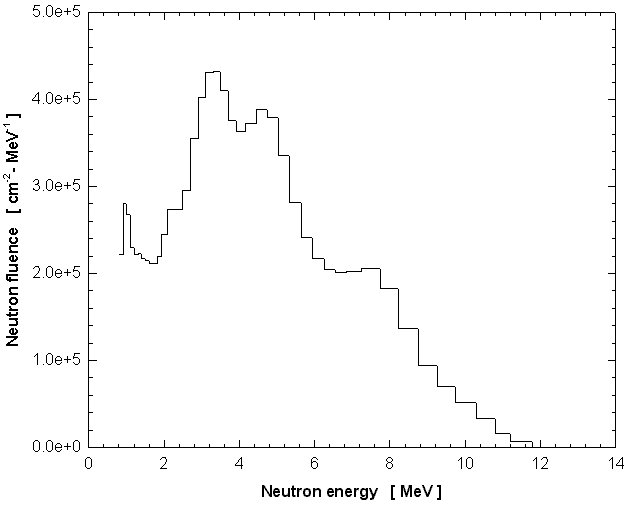
\includegraphics[width=0.7\textwidth]{images/239-PuBe-neutron-source-spectrum.png}
	\caption{Спектр нейтронів ізотопічного джерела з Pu та Be - мішенню} 
	\label{ris:neutron28Spectrum}	
\end{figure}
	
\newpage
\section{Постановка задачі}
\setcounter{figure}{0}
Метою даної роботи було створення моделі за допомогою якої можна було б отримати інформацію про елементи що входять до складу океанічного дна.
\subsection {Геометрії моделювання}
Змодельована геометрія схожа на ту яка використовувалась у проекті SABAT Рис. ~\ref{ris:SabatG}, але с наступними відмінностями: по-перше не моделювався корпус самої субмарини так як в він не ніс жодного корисного навантаження припроведені розрахунки, детектор та джерело були рознесені на дещо більшу відстань, та поміняні місцями, також на даному єтапі було вирішено відмовитись від моделювання морського дна, так як це дуже суттєва знижувало ефективність виконання коду. Також було приділено більшу увагу моделюванню захисту детектора.
\begin{figure}[hbt!]
	%\vspace{-10pt}
	\centering 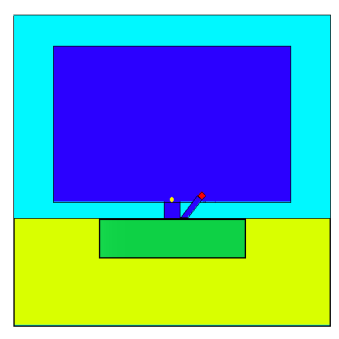
\includegraphics[width=0.7\textwidth]{images/sabatGeometry.png}
	\caption{Геометрія проекту SABAT} 
	\label{ris:SabatG}	
\end{figure}

Геометрія яка використовувалась для набору спектрів зображена на Рис. ~\ref{ris:Geometry}, довжина ребра куба середовища 1 м., довжина ребра бічної поверхні мішені (Рис. ~\ref{ris:Geometry} - 3 ) 40 см., від мішені до чутливого об'єму детектора 30 см., від чутливого об'єму до джерела 30 см., (відстані задані не враховуючи зовнішній захист) матеріал середовища був взятий с запропонованою бази матеріалів Geant4 - "G4\_WATER". Джерело нейтронів поміщене в направляючий об'єм(Рис. ~\ref{ris:Geometry} - 1), який виготовлений з тонкого шару свинцю. Чуттєвий об'єм детектора поміщений у захист зі свинцю, бору, та алюмінія, направляючі об'єми заповнені повітрям(G4\_AIR)
\begin{figure}[hbt!]
	%\vspace{-10pt}
	\centering 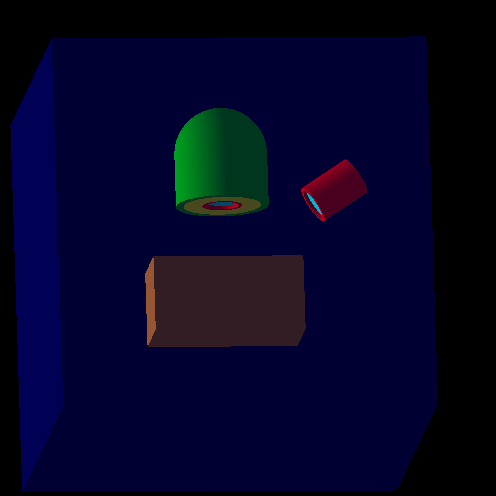
\includegraphics[width=0.7\textwidth]{images/geometryAll.png}
	\caption{Геометрія моделі, 1 - джерело і його направляючий об'єм, 2 - захист детектора та детектор, 3 - мішень} 
	\label{ris:Geometry}	
\end{figure}

Для спрощення моделювання точкове джерело нейтронів було розміщенне всередині набравляючого кооксіального об'єму Рис. ~\ref{ris:Geometry} (червоного кольору), під кутом для того щоб більша кількість нейтронів потрапляла в поверхню яка безпосередню знаходиться під чутливим об'ємом детектора 
	
	
	\subsection{Чутливий об'єм детектора та захист}
	
	Для моделювання чутливого об'єму був обраний надчистий германій, з діаметром 60.6 міліметрів, та довжиною 56.7 міліметрів. Рис. ~\ref{ris:s_detector_volume} 	
	\begin{figure}[hbt!]
		%\vspace{-10pt}
		\centering 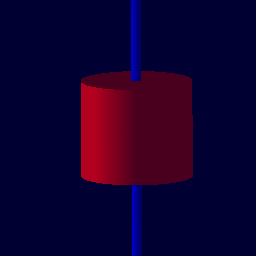
\includegraphics[width=0.7\textwidth]{images/sDetector158cm3.png}
		\caption{Форма чутливого об'єму} 
		\label{ris:s_detector_volume}	
	\end{figure}
	
	Детектор буде розміщенний поряд з джерелом нейтронів високих енергій, 14.2 МеВ. Тому детектор був розміщений у трьох шаровий захист. Рис. ~\ref{ris:s_detector_P}	
	\begin{figure}[hbt!]
		%\vspace{-10pt}
		\centering 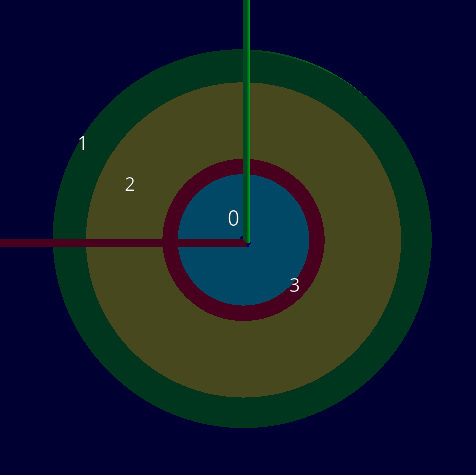
\includegraphics[width=0.7\textwidth]{images/dectorPrt.png}
		\caption{Захист детектора, Al - 1 (зелений) товщина 2 см., B - 2 (жовтий) товщина 5 см., Pb - 3 (червоний) товщина 1 см. 0 (Блакитний) шар повітря} 
		\label{ris:s_detector_P}	
	\end{figure} 
	
	В захисті використовується Бор для поглинання теплових нейтронів, так як вся детекторна система буде знаходитися під водою, то нейтрони від джерела будуть втрачати енергію при пружному розсіянні на водню. 
	
	Для поглинання теплових нейтронів перед чутливим об'ємом детектора був обраний $B^{10}$. Використовується в ПВЕЛ-ах для контролю кількості теплових нейтронів в активній зоні реакторної установки ВВЕР. 
	$B^{10} ( n, \alpha \gamma)Li_3^7$, Переріз захоплення нейтрона $B^{10} \ \sigma = 3380$ барн.
	$E_\gamma$ = 480 кеВ, реакція з вильотом $\gamma$ - кванту протікає з ймовірністю 94\%.
	
	Для зовнішнього корпусу захисту чутливого об'єму використовувався $Al^{26}$ - товщиною 1 см на Рис. ~\ref{ris:s_detector_P} - зоображений зеленим кольором 
	
	За приклад було взято детектор N21879A виробника від ORTEC AMETEK, параметри розмірів були взяті від офіційного дистриб'ютора.
	\subsection{Досліджувані речовини} 
	
	
	В рамках данного моделювання були розглянуті матеріали розглянуті в Таб.~\ref{tabl:Materials}.
	\begin{table}[h]
		\centering
		\caption{Елементи та ізотопи які входять до їх складу} 
		\begin{tabular}{|c|c|c|}
			\hline
			Назва & Хімічна склад & Ізотопний склад \\
			\hline
			Гірчичний газ & $C_4H_8Cl_2S$ & $C^{12}$, 	$H^1$, $Cl^{35}$, $S^{22}$ \\
			\hline
			Ютенбогардтит & $Ag_3AuS_2$ & $Ag^{108}$ , $Au^{197}$ , $S^{32}$ \\
			\hline
			Халькопірит & $CuFeS_2$ & $Cu^{64}$, $Fe^{56}$, $S^{22}$ \\
			\hline
			Збіднений уран & U & 99.27\% $U^{238}$, 0.7\%$U^{235}$, 0.005\%$U^{234}$\\
			\hline
		\end{tabular}
		\label{tabl:Materials}
	\end{table}
	
	Найбільш інтенсивні піки для кожного з елементів розглянуті в Табл. ~\ref{tabl:ElementsEnergy}, використовувались елементи з бази доступної в Geant4
	\begin{table}[h]
		\centering
		\caption{Таблиця енергій найбільш інтенсивних піків} 
		\begin{tabular}{|c|c|} 
			\hline
			Елемент& Енергія, МеВ \\
			\hline
			$Cl$ & 0.79, 1.17, 1.94, 2.12, 6.12, 7.79, 8.58 \\
			\hline
			$H$ & 2.23 \\
			\hline
			$C$ & 4.44 \\
			\hline
			$Fe$ & 7.64, 9.30 \\		
			\hline
			$S$ & 2.96, 4.73 \\
			\hline
			$Cu$ &  \\
			\hline
			$U$ & 1.26\\
			\hline
			$Ag$ &  0.74, 6.26 \\
			\hline
			$Au$ & 0.67, 1.087, 2.24, 1.37  \\
			
			\hline
		\end{tabular}
		\label{tabl:ElementsEnergy}
	\end{table}
	
	\subsection{Код моделі}
	Ціллю було написати максимально зручний код для набору спектрів за різних умов та на різних мішенях, тому були створені абстрактні класси для створення геометричних об'єктів. Для зручності створення матеріалів були створенні структури. 
	Та для пришвидшення роботи були всі можливі константи ініціалізувалися на етапі компіляції. Для полегшення контролю над пам'яттю використовувалися розумні вказівники С++ 14 стандарту. Архітектура коду моделювання зоображена на Рис. ~\ref{ris:s_classDiagram} 
	\begin{figure}[hbt!]
		%\vspace{-10pt}
		\centering 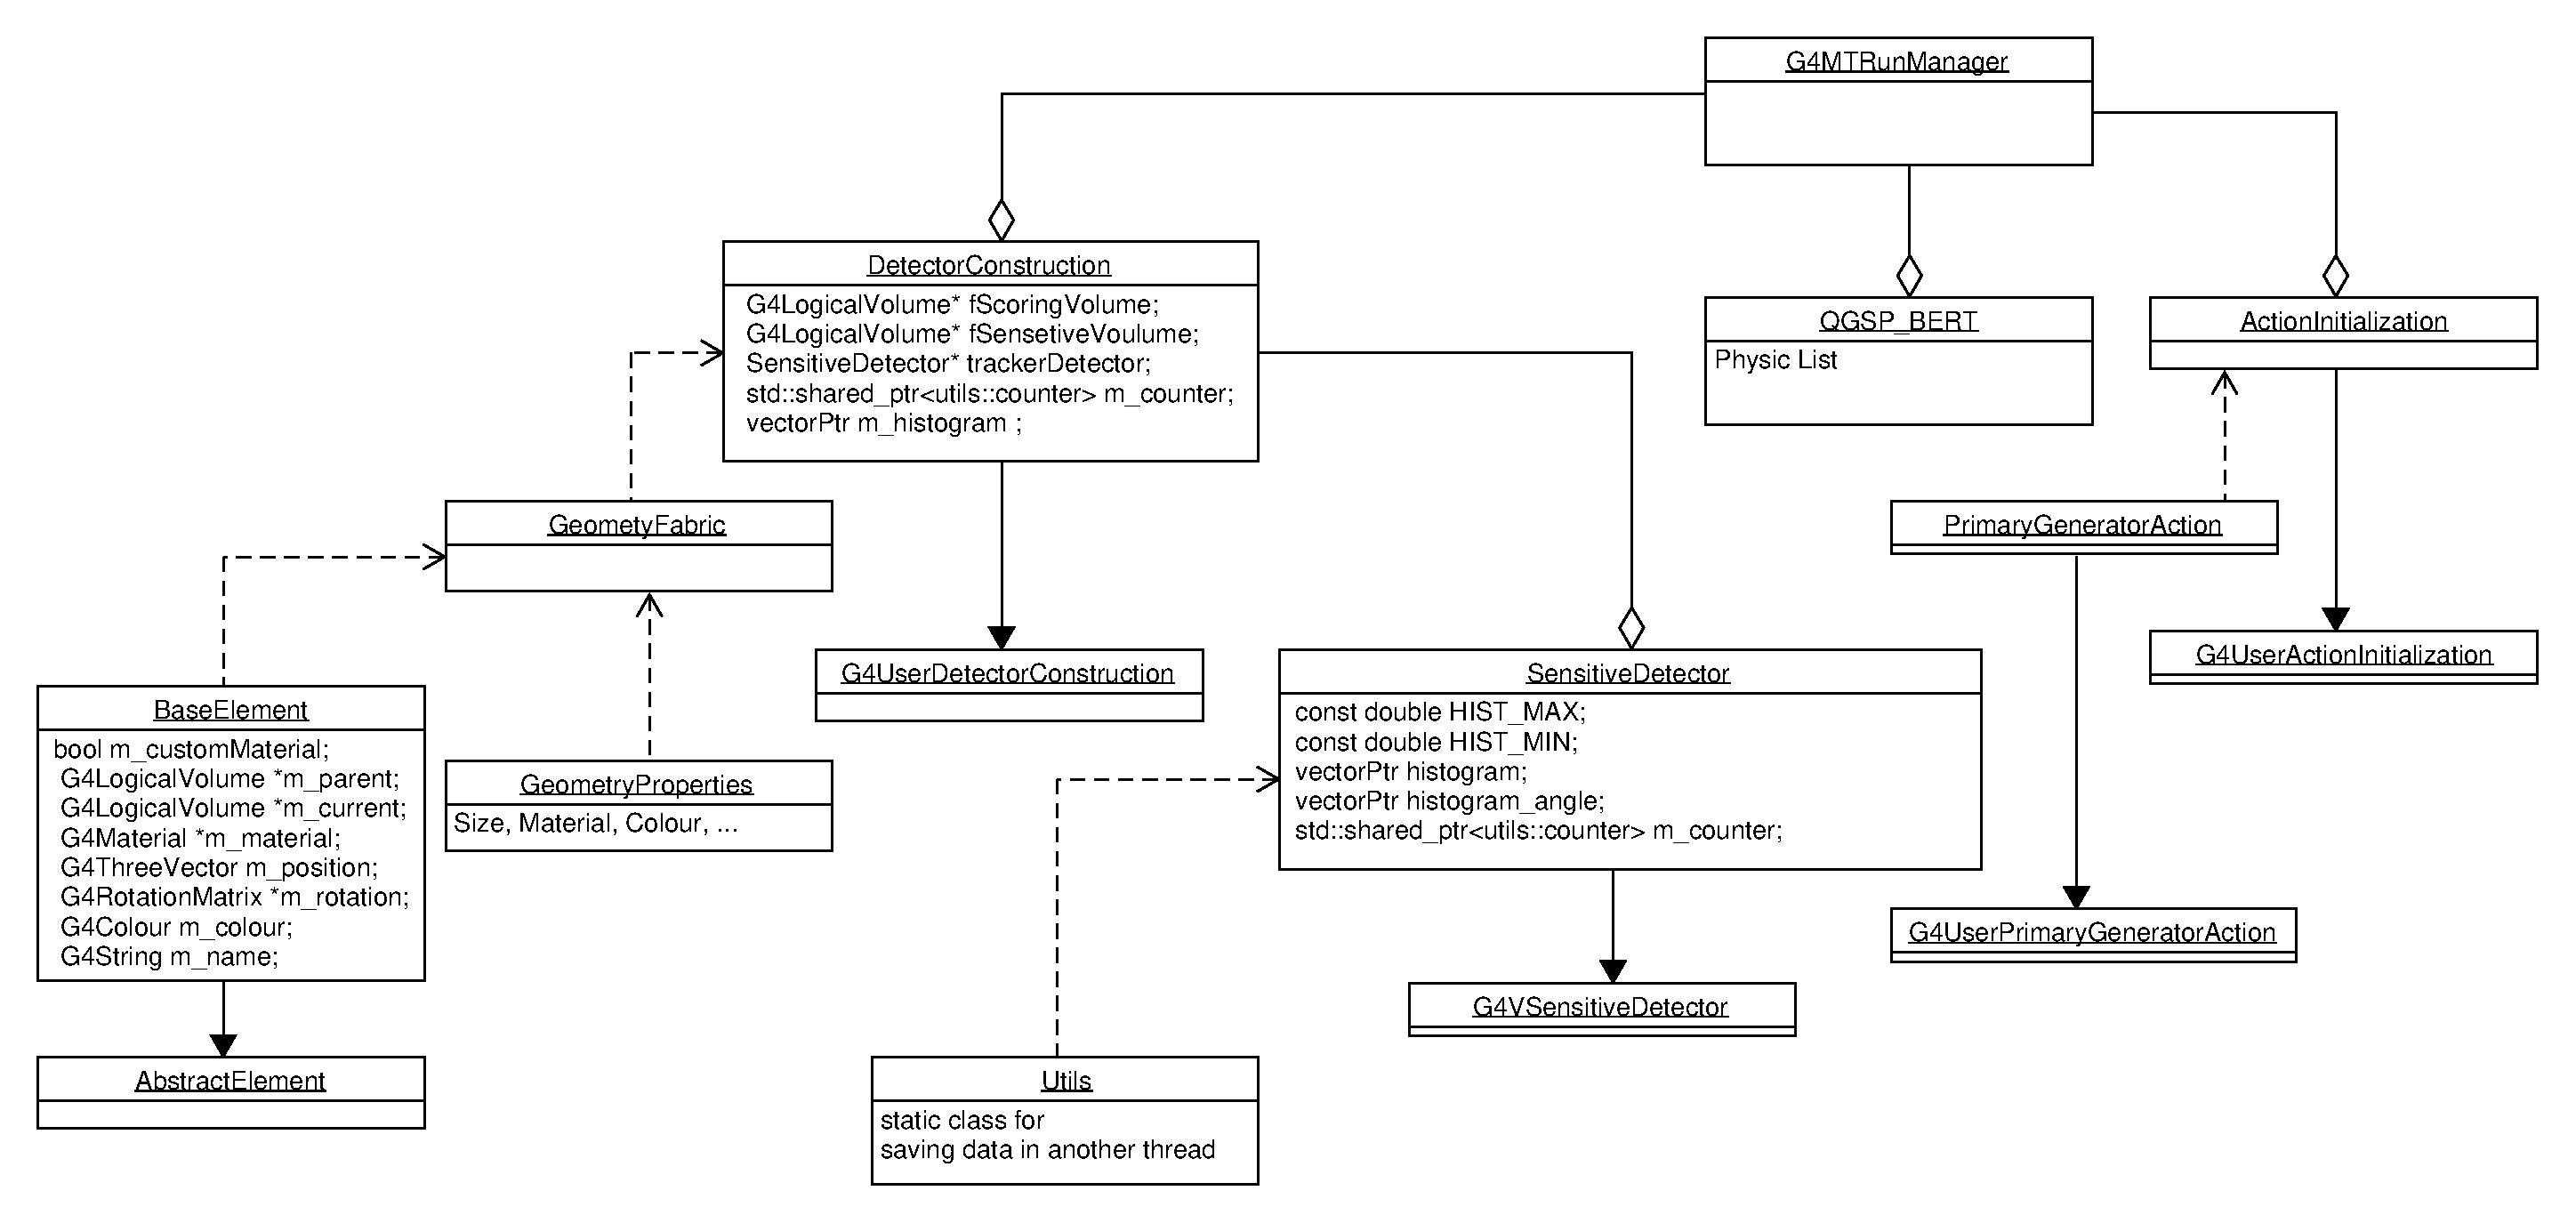
\includegraphics[width=1\textwidth]{res/classDiagram.pdf}
		\caption{Діаграма класів коду моделі} 
		\label{ris:s_classDiagram}	
	\end{figure} 
	Проаналізувавши різницю між двома фізичними моделями $QGSP\_BERT\_HP$ та $QGSP\_BERT$, для проведення моделювання була обрана $QGSP\_BERT$ - так як на данному єтапі вона виявилась більш підходящою, через вищу продуктивність.
	
	
	\newpage 
	\section{Аналіз результатів}
	\setcounter{figure}{0}
	\subsection{Опис обробки спектру}
	
	В результаті моделювання, чутливим об'ємом набирались апаратні спектри, для чутливого об'єму було встановлено 16384 біни. Далі для наближення спектру до реального, була проведене його сглажування за наступної формулою $\Delta{E} = 2.36 \sqrt{F  \frac{w}{E}}  w$, $\Delta{E}$ - енергія на один бін, F - Фано фактор, w - кількість енергії на утворення пари, та про нормований на кількість нейтронів з джерела. Так як для спрощення побудови джерела в моделі, використовувалась спрощена геометрія, а генерація нейтронів відбувалися майже строго у заданому напрямку. Так як джерело нейтронів вважалося ізотропним, то загальна кількість частинок розраховувалась наступною формулою $ 4 \pi n = N$, де $N -$ це загальна кількість частинок. В моїй роботі для згладжування спектру були взяті наступні параметри Табл. ~\ref{tabl:Param}
	\begin{table}[h]
		\centering
		\begin{tabular}{|c|c|c|} 
			\hline
			Параметр & Значення &  Розмірність \\
			\hline
			$F$ & 0.13 & - \\
			\hline
			$w$ & 3.62 & eV \\		
			\hline
		\end{tabular}
		\caption{Таблиця значень для уширення піків} 
		\label{tabl:Param}
	\end{table}
	\begin{figure}[hbt!]
		%\vspace{-10pt}
		\centering 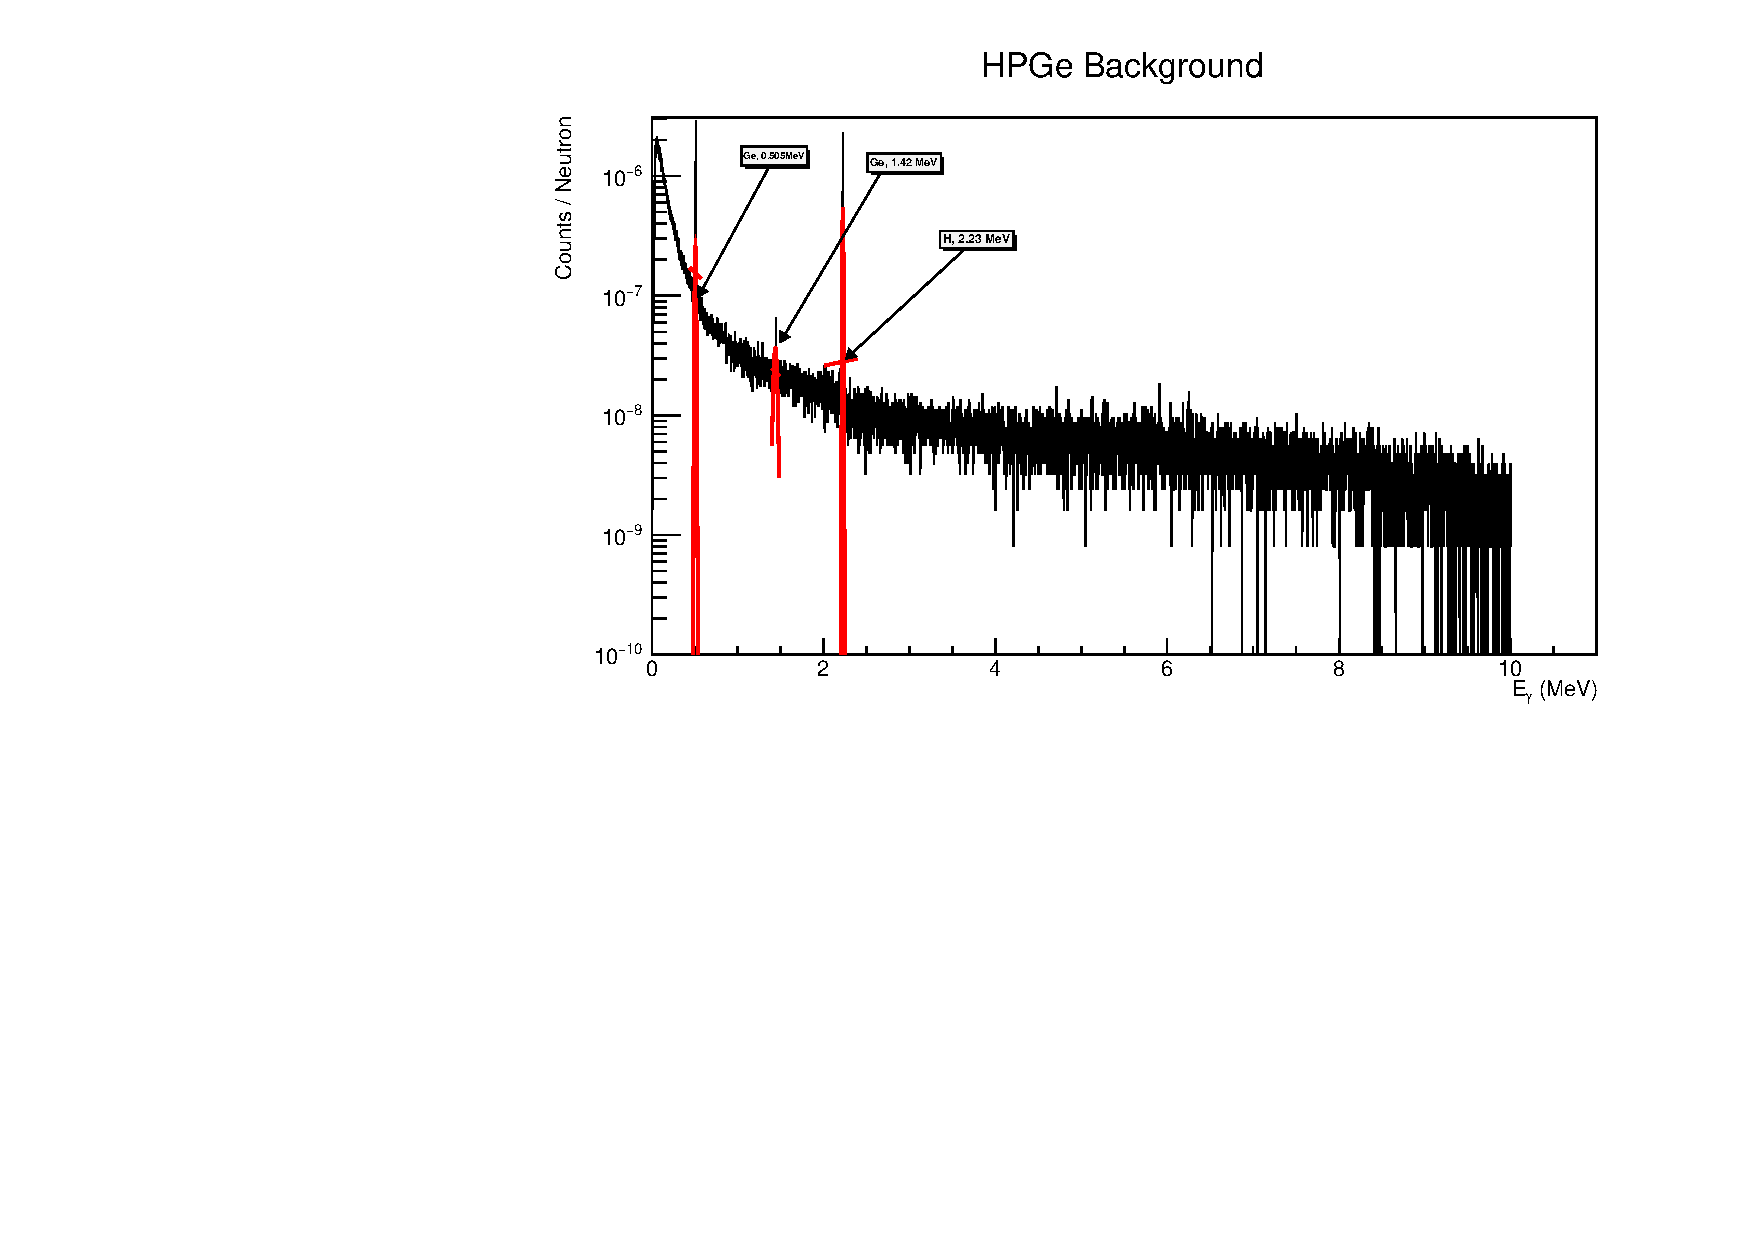
\includegraphics[width=1\textwidth]{res/background.pdf}
		\caption{Фон} 
		\label{ris:FonPicks}	
	\end{figure} 
	
	Фон Рис. ~\ref{ris:FonPicks} набрався за тої самої геометрії Рис. ~\ref{ris:SabatG}, але за відсутності мішені(коричневий паралелепіпед), У фоні були проаналізовані наступні три піки: H з $E_\gamma = 2.23 MeV$, та два піки які отримали за рахунок захоплення теплових нейтронів $Ge$ з $E_\gamma = 0.505MeV$, $E_\gamma = 1.42 MeV$ - це означає що даної геометрії частина нейтронів від джерела проходячи через захист потрапляє в чутливий об'єм детектора, та призводить до його руйнації. Дані піки відповідають пікам $Ge^{72}(n, \gamma)Ge^{73}$ - реакції з нейтронами енергій близькими до теплових - $E_n = 0.025eV$. $Ge^{72}$ - основний ізотоп Ge, і саме він використовується в основі чутливого об'єму.
	\begin{table}[h]
		\centering
		\begin{tabular}{|c|c|c|c|} 
			\hline
			$E_{\gamma}$, MeВ & $\Delta{E}$, МеВ & $I = I_{\gamma} / I_{b}$ & $\Delta{I}$\\
			\hline
			0.505 & 0.008 & 12 & 3 \\
			\hline
			1.420 & 0.004 & 20 & 4 \\	
			\hline
			2.230 & 0.003 & 22 & 4 \\	
			\hline
		\end{tabular}
		\caption{Фонові піки} 
		\label{tabl:ResultsBackground}
	\end{table}
	
	\subsection{Валідація моделі}
	
	Для підтвердження можливості проведення наборів на моїй моделі був набраний спектор для Гірчичного газу ($C_4H_8Cl_2S$). Рис ~\ref{ris:MustBackAllLogSm}. Та порівняний з отриманим спектром набраним задопогою коду для моделювання MCNP в проекті SABAT.
	\begin{figure}[hbt!]
		%\vspace{-10pt}
		\centering 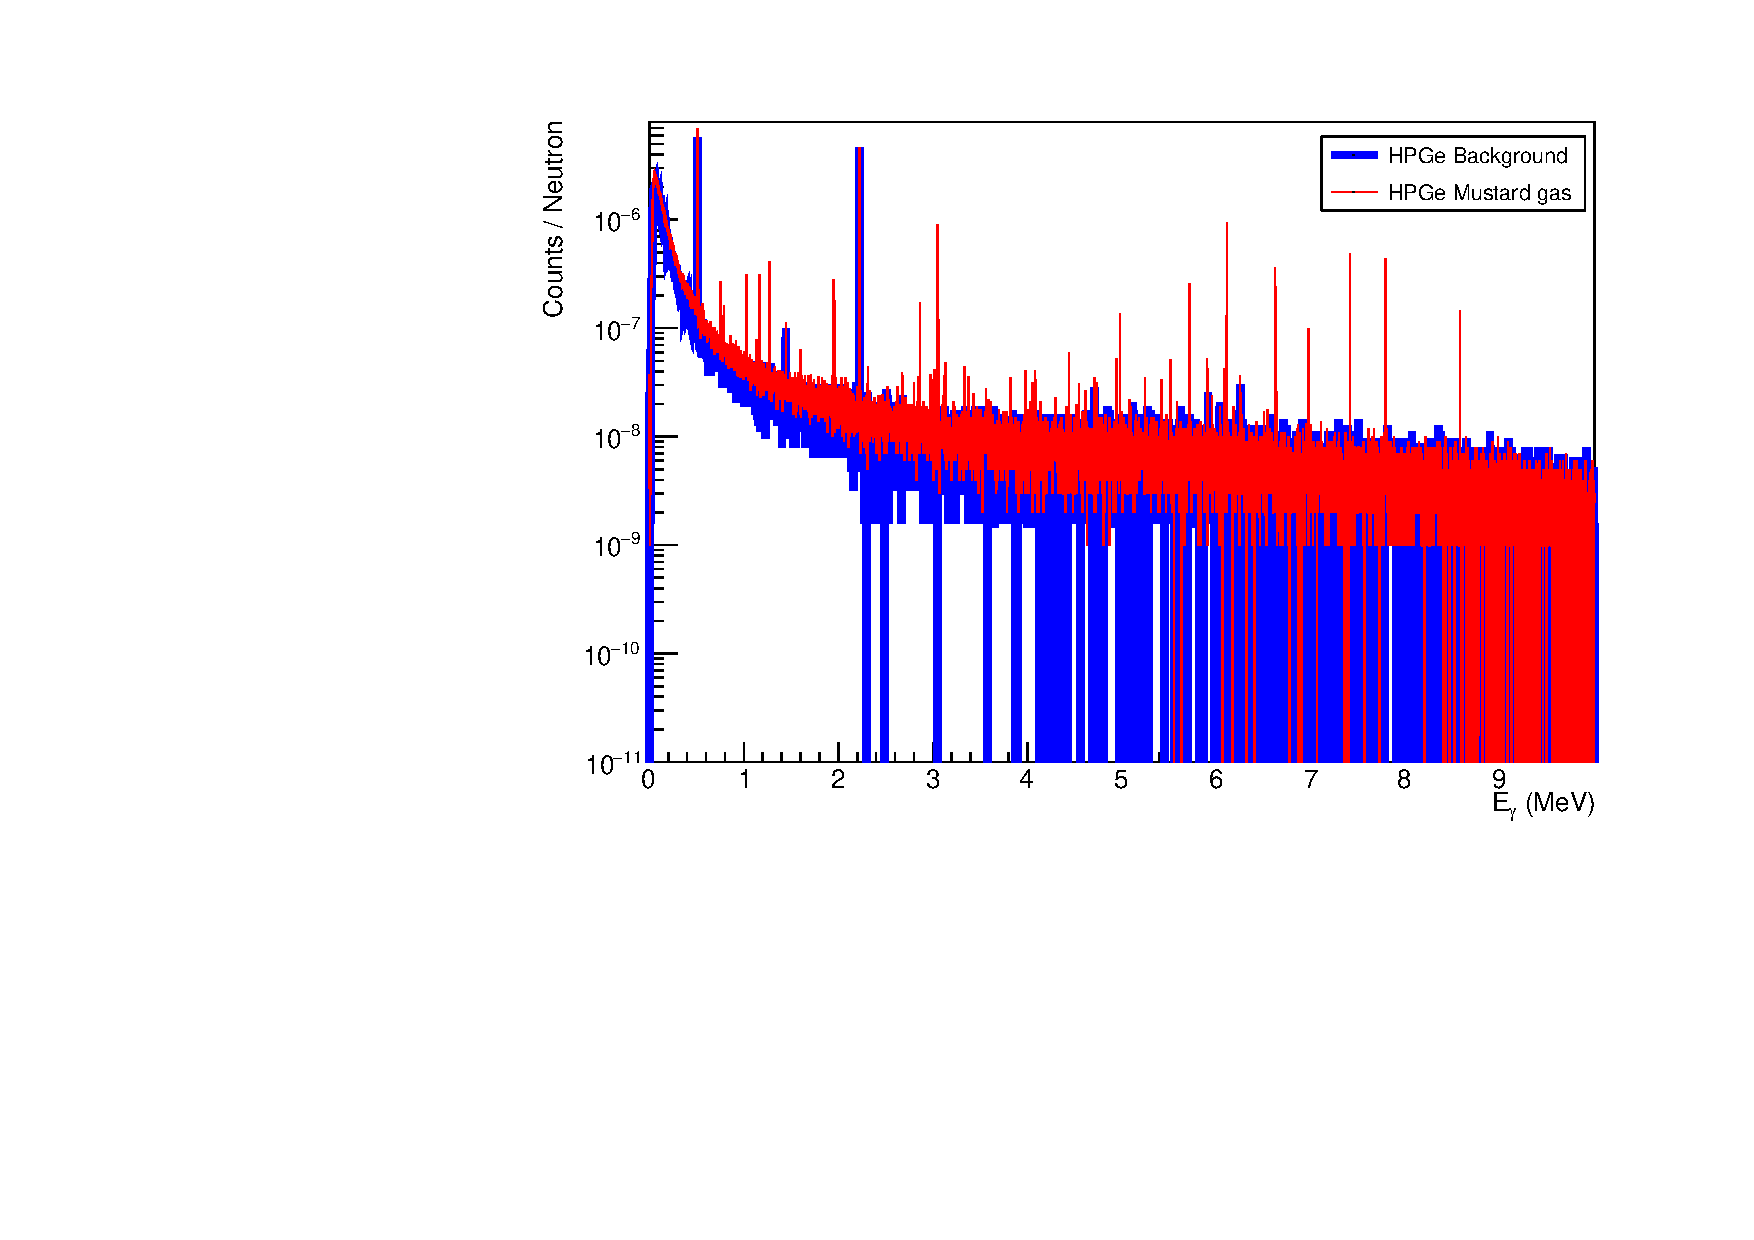
\includegraphics[width=1\textwidth]{res/smMustFonAll.pdf}
		\caption{Червоним - представлений спектр для Гірчичного газу. Синім - фону} 
		\label{ris:MustBackAllLogSm}	
	\end{figure} 
	Це спектор набрався для валідації моделі - тому до уваги бралися лише ті піки, які були вказані в проекті SABAT. Табл. ~\ref{tabl:ResultsMustard}
	\begin{table}[h]
		\centering
		\begin{tabular}{|c|c|c|c|c|} 
			\hline
			$E_{\gamma}$, MeВ & $\Delta{E}$, МеВ & $I = I_{\gamma} / I_{b}$ & $\Delta{I}$ & Елемент\\
			\hline
			0.79 & 0.008 & 12 & 3 & Cl\\
			\hline
			1.165 & 0.004 & 20 & 4 & Cl \\	
			\hline
			1.95 & 0.003 & 22 & 4 & Cl \\	
			\hline		
			4.44 & 0.003 & 22 & 4 & C \\	
			\hline
			7.41 & 0.003 & 22 & 4 & Cl\\	
			\hline
			7.78 & 0.003 & 22 & 4 & Cl\\	
			\hline			
			8.58 & 0.003 & 22 & 4 & Cl\\	
			\hline
		\end{tabular}
		\caption{Піки гірчичного газу - $C_4H_8Cl_2S$} 
		\label{tabl:ResultsMustard}
	\end{table}
	
	\begin{figure}[hbt!]
		%\vspace{-10pt}
		\centering 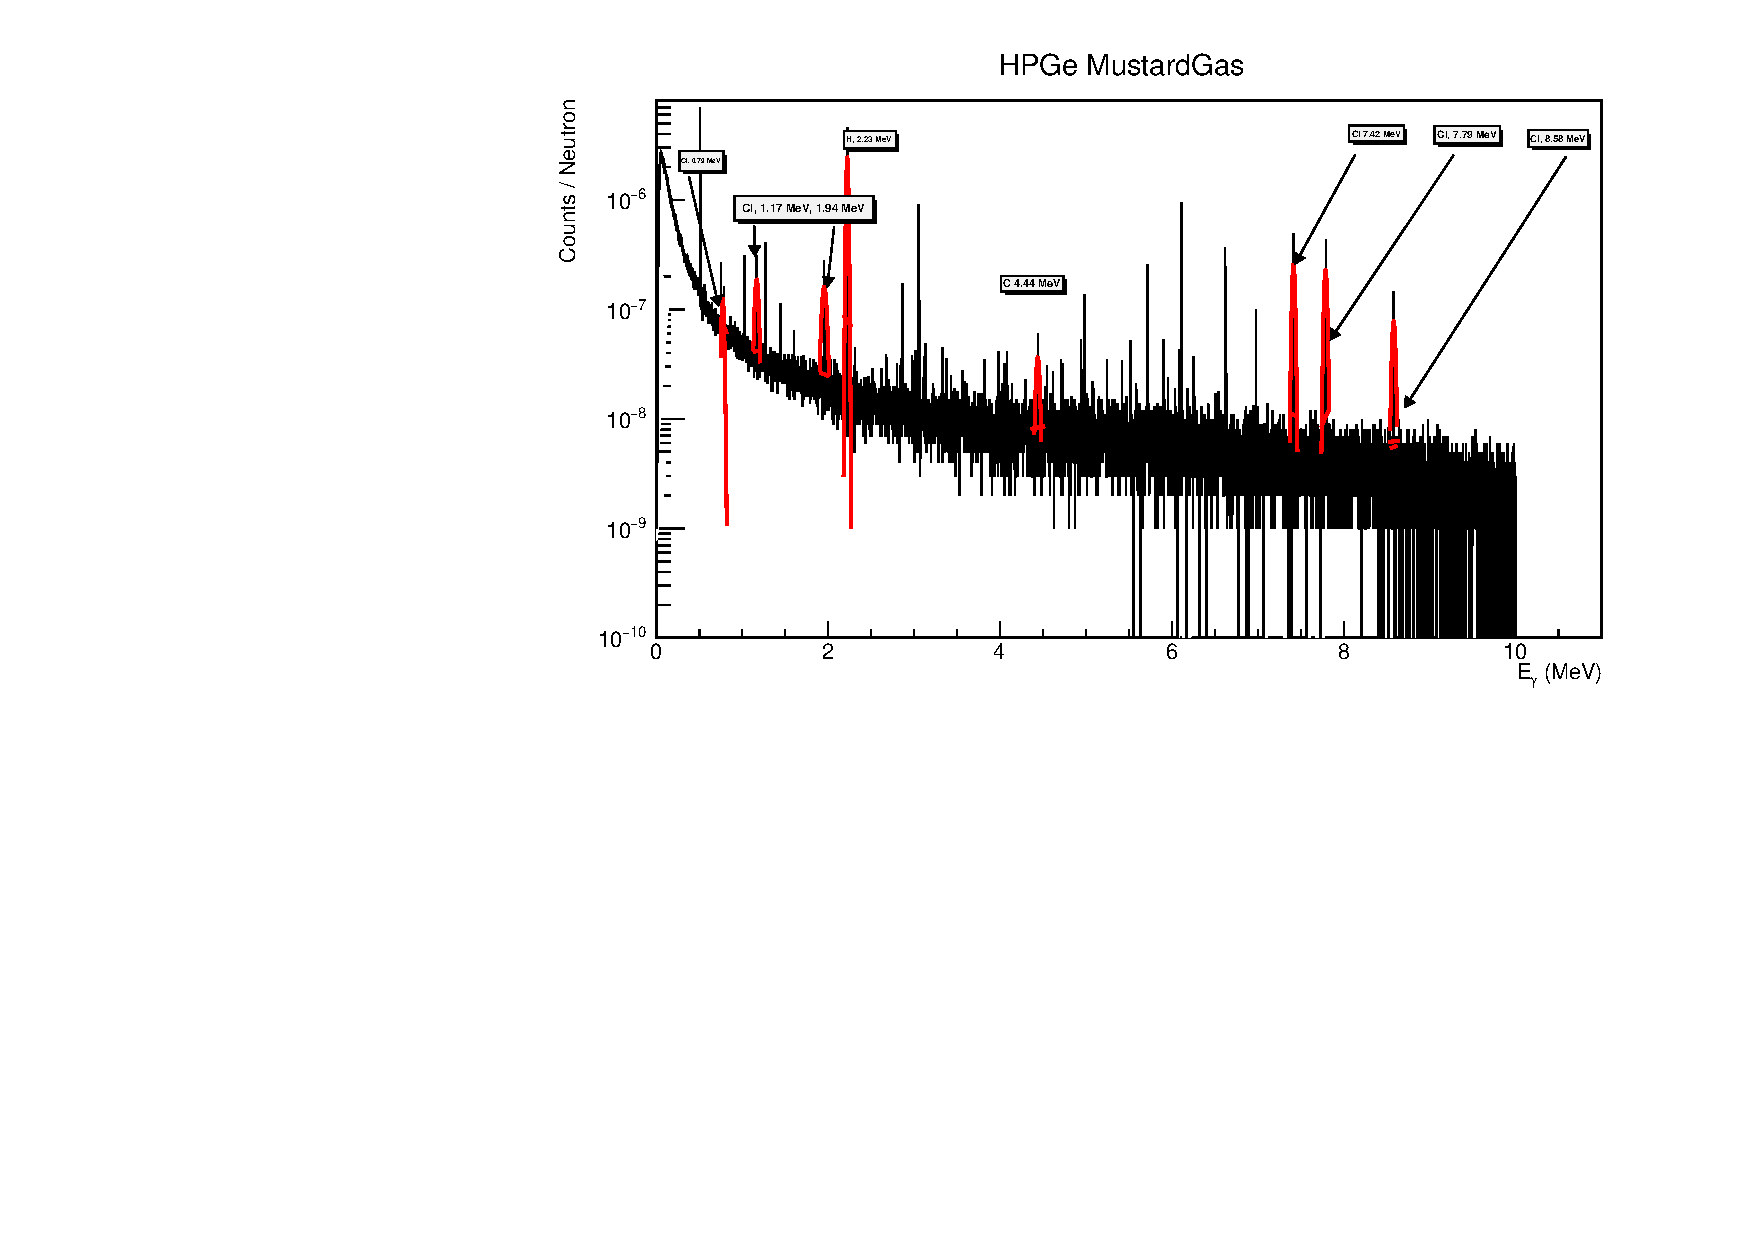
\includegraphics[width=1\textwidth]{res/mustard_gas.pdf}
		\caption{Ініціалізація піків, Cl, H, C - в спектрі гірчичного газу} 
		\label{ris:mustard}	
	\end{figure} 
	
	\subsection{Дослідження $(n, \gamma)$ реакцій, Au та Cu} 
	$Au^{197}(n,\gamma)Au^{198}$ - реакція захоплення нейтрона, переріз захоплення нейтронів в залежності від енергії зображено на Рис.~ \ref{ris:AuSigma}.
	\begin{figure}[hbt!]
		%\vspace{-10pt}
		\centering 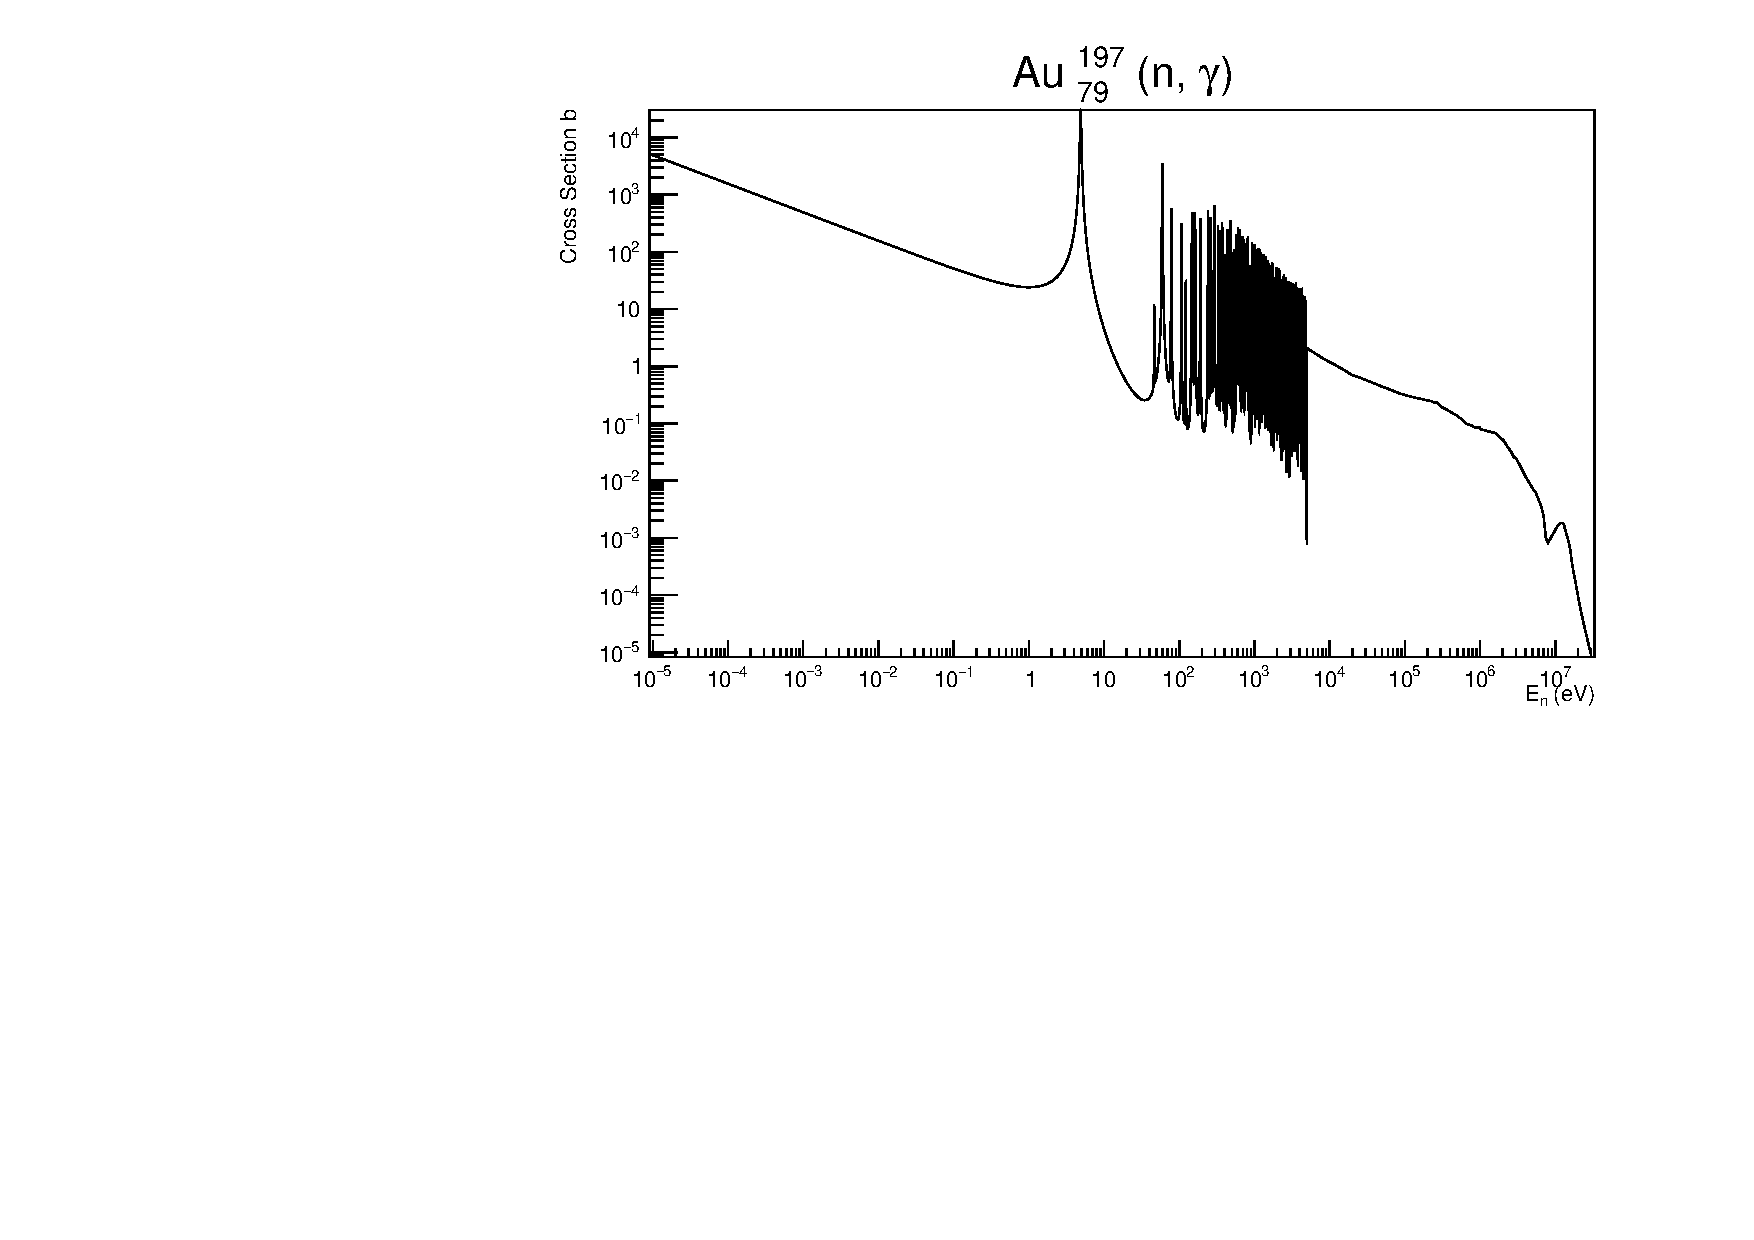
\includegraphics[width=1\textwidth]{sigma/Au197Sigma.pdf}
		\caption{Залежність захоплення нейтрона від енергії нейтронів в реакції  $Au^{197}(n,\gamma)Au^{198}$} 
		\label{ris:AuSigma}	
	\end{figure} 
	
	$Au^{198} $ - ізотоп, має 2 - рівні в результаті розпаду з яких випромінюється гамма кванти, $T_{1/2} = 2.6$ днів. На Рис. \ref{ris:Au198Level12-} зображено перехід з збудженого $J\pi$ 12- на $J/\pi$ 2- з якого у данного ізотопа відбувається $\beta^-$ розпад до стабільного $Hg^{198}_{80}$.
	
	$Hg^{198}$ - має два збудженні рівні $J\pi$ 2+ - перехід з  в основний стан відбувається з випромінення $\gamma$-кванту $E_\gamma=1087keV$, каскадний перехід є основним с способом переходу на стабільний рівень $Hg^{198}$, відбувається з випромінення двох $\gamma$-квантів $E_\gamma$ = 675 кеВ та $E_\gamma$ = 411 кеВ. 
	
	На Рис. ~\ref{ris:AuSigma} - гарно видно що є резонансна область поглинання нейтронів розтягується до декількох кеВ. 
	\begin{table}[h]
		\centering
		\begin{tabular}{|c|c|c|c|c|} 
			\hline
			$E_{n}$, eВ&$E_{\gamma}$, кеВ & $\Delta{E_{\gamma}}$, кеВ & $I_{\gamma} / 100_n$ & $\Delta{I}$ \\
			\hline
			4.9 & 6252.6 & 0.7 & 40.0 & 1.6 \\
			\hline
			4.9 & 6457.8 & 0.7 & 20.4 & 0.5\\	
			\hline
			4.9 & 5710.7 & 0.7 & 10.1 & 0.7 \\	
			\hline	%60.        6061.3      0.9        16.2   -01  1.5 	
			60 & 6061.3 & 0.9 & 16.2 & 1.5 \\	
			\hline % 5710.7      0.7        16.0   -01  1.5   -01
			60 & 5710.7 & 0.7 & 16.0 & 1.5 \\	
			\hline % 78.        4958.2      1.0        10.5   -01  0.6   -01
			78 & 4958 & 1.0 & 10.5 & 0.6\\	
			\hline% 107.       5808.2      0.9        17.3   -01  1.0   -01
			107 & 5808.2 & 0.9 & 17.3 & 1.0 \\	
			\hline
		\end{tabular}
		\caption{$E_\gamma$, для нейтронів з енергіями поблизу резонансної області для $Au^{197}$} 
		\label{tabl:AuNeutronAbsorption}
	\end{table}
	
	В реакція $Cu^{64}(n, \gamma)Cu^{65}$ переріз захоплення теплового нейтрона $\sigma$ = $2.1 \times 10^3 \pm \ 1.9 \times 10^3$ барн. $Cu^{65}$ - стабільний елемент. $Cu^{65}(n,\gamma)Cu^{66}$.
	\begin{figure}[hbt!]
		%\vspace{-10pt}
		\centering 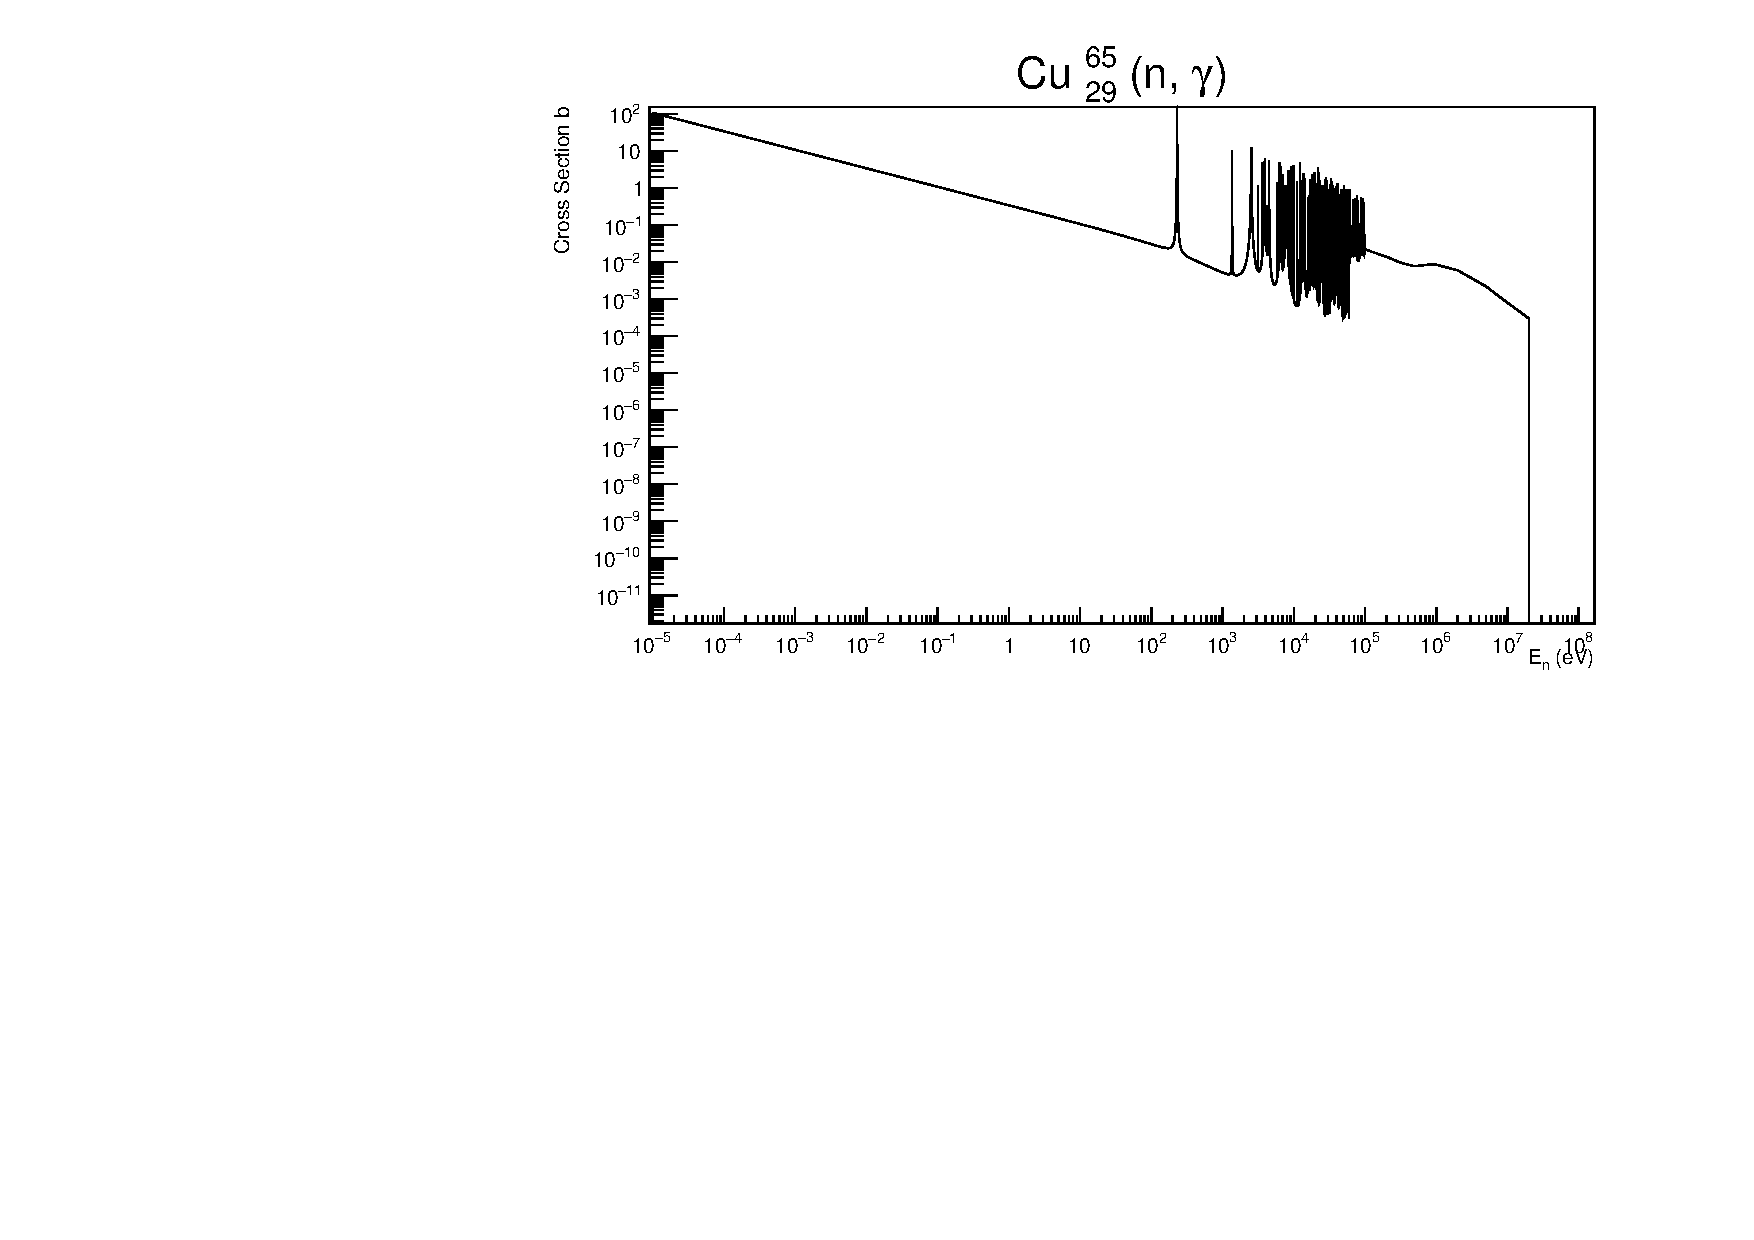
\includegraphics[width=1\textwidth]{sigma/Cu65Sigma.pdf}
		\caption{Залежність захоплення нейтрона від енергії нейтронів в реакціїї  $Cu^{65}(n,\gamma)Cu^{66}$} 
		\label{ris:CuSigma}	
	\end{figure} 
	Для данного изотопу спостерігається існування резонансної області в діапазоні десятків кеВ Рис. ~\ref{ris:CuSigma}. 
	$Cu^{66}$ - не стабільний ізотоп, якому притаманний $\beta^-$ розпад в $Zn^{66}_{30}$, $T_{1/2} = 5.12$ хвилин. 
	$Zn^{66}$ - стабільний ізотоп з основним рівнем $J\pi$ 0+. $\beta^-$ - розпад $Cu^{66}$ в основному відбувається у стабільний стан, але є ймовірність розпаду на $J\pi$ 1+ рівень, з подальшим випромінення $\gamma$ - кванту з енергією $E_{\gamma} = 1039$ кеВ. Рис. ~\ref{ris:ZnLevels-}
	\\
	\subsection{Аналіз спектрів $Ag_3AuS_2$}
	За матеріал було обрано ютенбогардтит $Ag_3AuS_2$ - родовища з даними мінералами були знайдені на камчатці поблизу узбережжя. Данний мінерал відноситься до рідкисних золотоносних руд, зустрічаеться в природі у твердому стані. Був знайдений на Камчатських родовищах. Рис. ~\ref{ris:Ag3AuS2Fon}		
	\begin{figure}[hbt!]
		%\vspace{-10pt}
		\centering 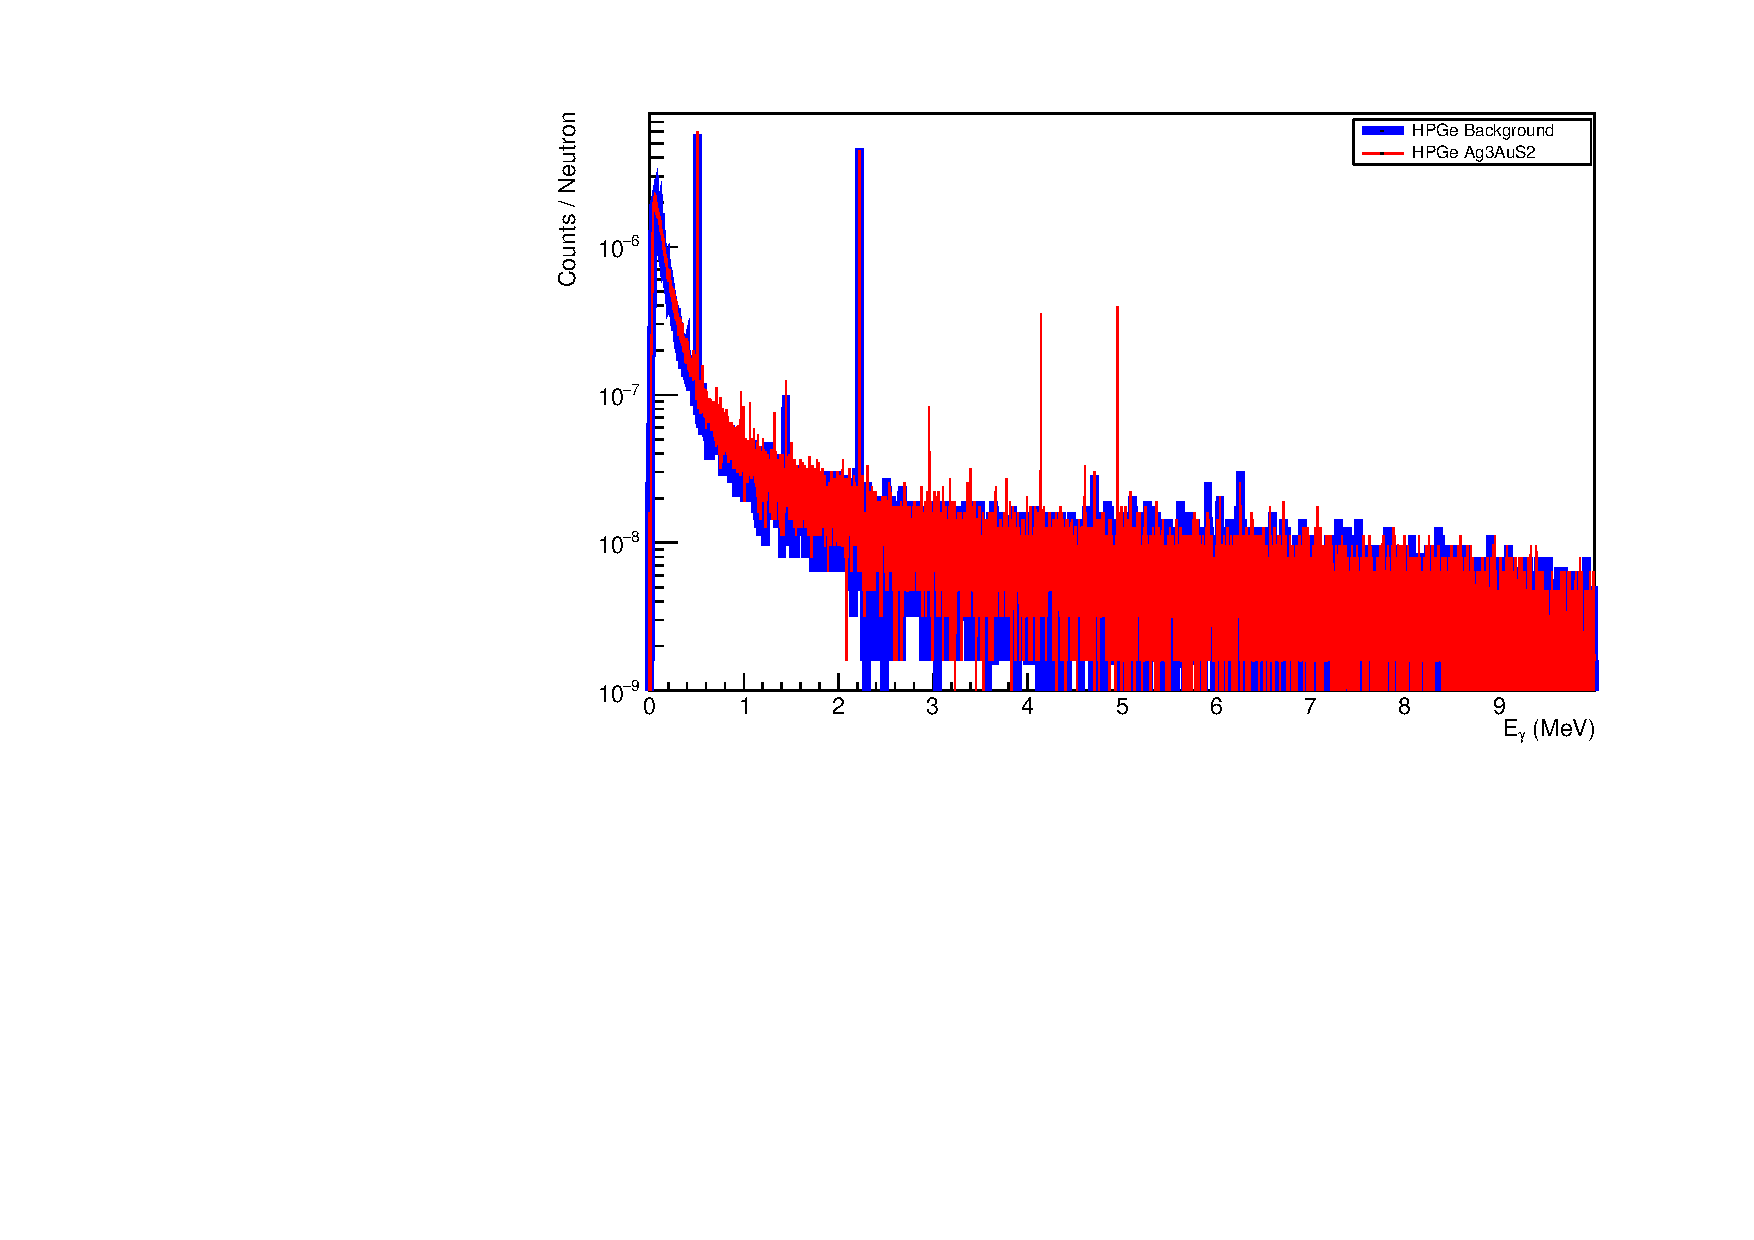
\includegraphics[width=1\textwidth]{res/auFonAllLog.pdf}
		\caption{Червоним - представлений спектор для $Ag_3AuS_2$. Синім - фону} 
		\label{ris:Ag3AuS2Fon}	
	\end{figure} 	
	Даний спектор і фон були набрані при опроміненні нейтронами з джерела максимальної енергією 14.2 МеВ
	Для порівняння було проведено опромінення за допомогою нейтронів енергією 8.5 та 2.8 МеВ. Рис. ~\ref{ris:Ag3AuS28_5MeV}	
	В набраному спектрі при енергіях нейтронів з джерела 8.5 МеВ, були проаналізовані наступні піки
	\begin{figure}[hbt!]
		%\vspace{-10pt}
		\centering 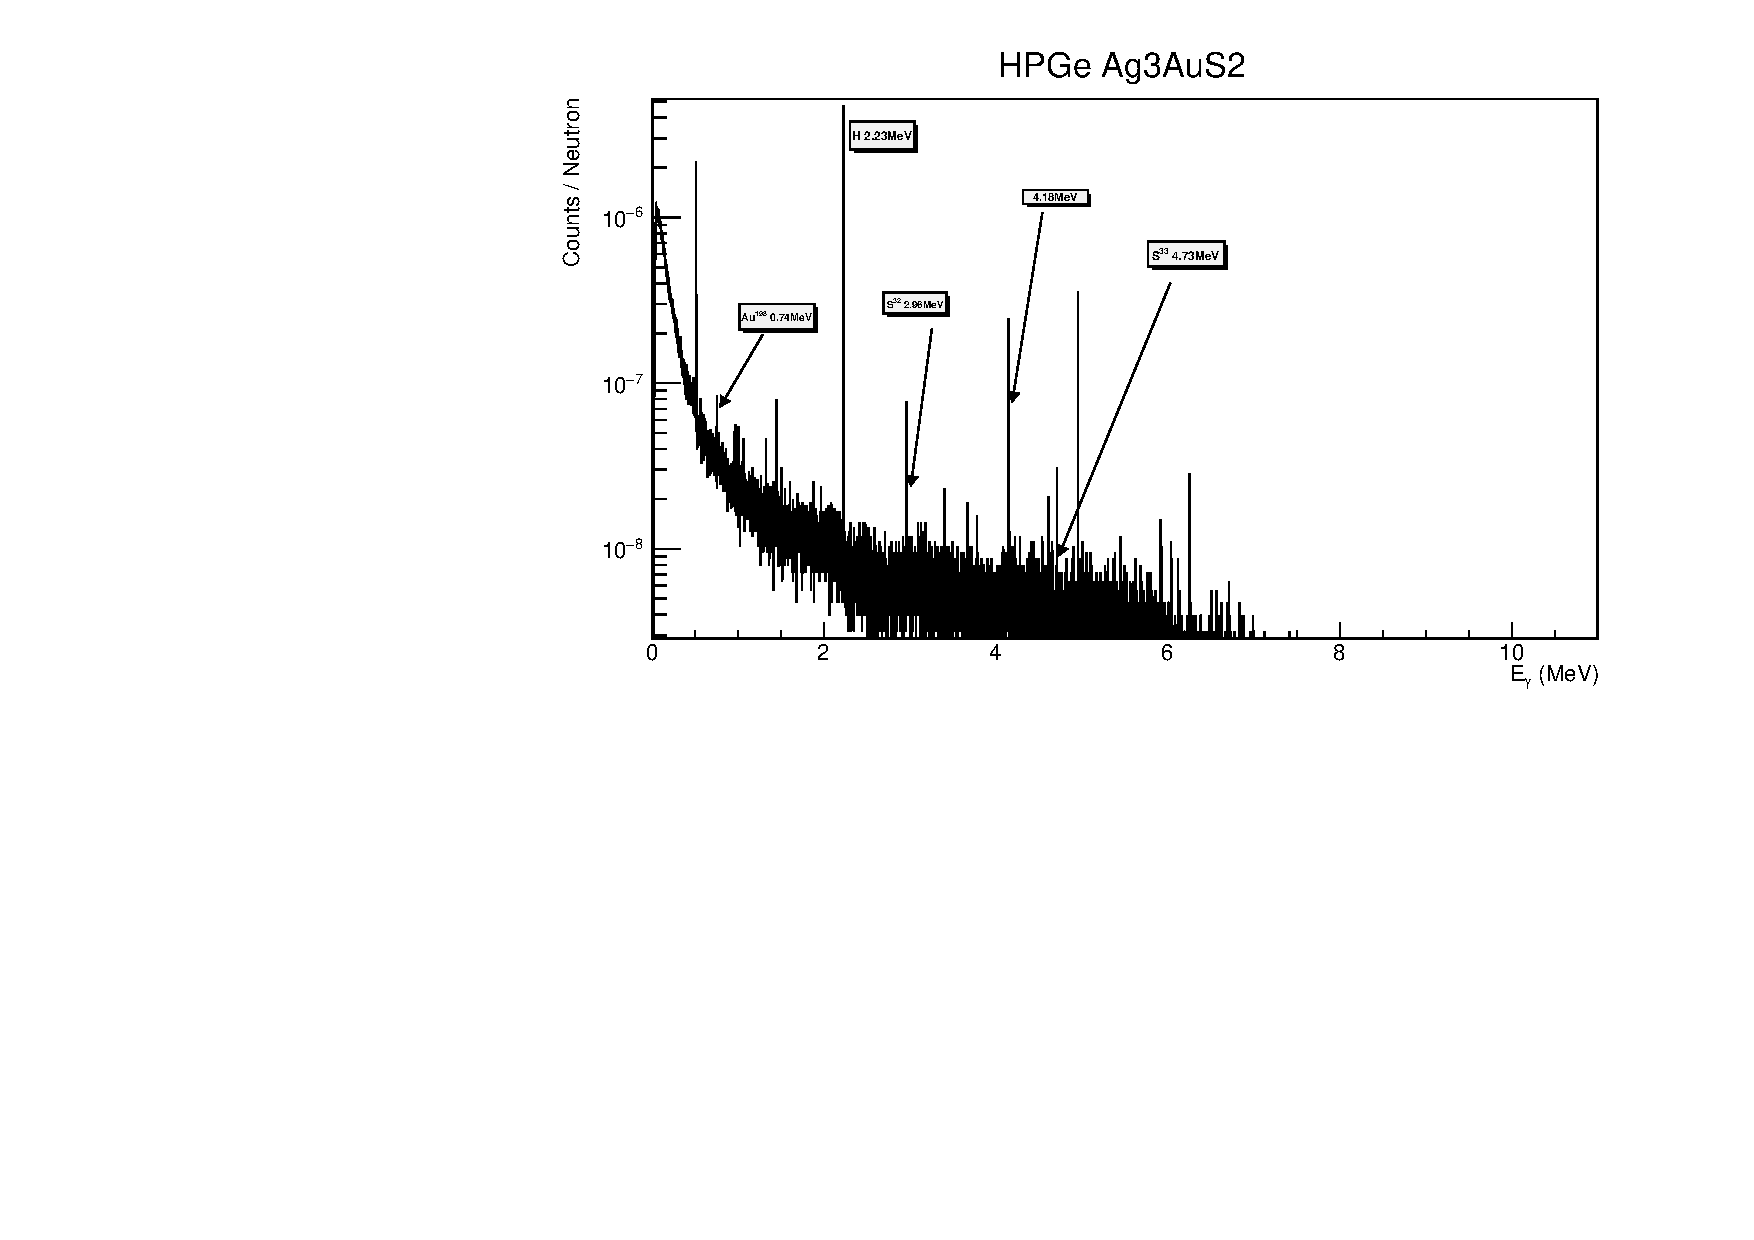
\includegraphics[width=1\textwidth]{res/Au_AnzSpectr.pdf}
		\caption{Спектор $Ag_3AuS_2$, $E_{n} = 8.5 MeV$ - енергія нейтронів з джерела}
		\label{ris:Ag3AuS28_5MeVPick}	
	\end{figure} 
	Для того щоб проаналізувати залежність можливості використання ізотопних джерел був набраний спектор, за енергій нейтронів 2.8 МеВ Рис. ~\ref{ris:Ag3AuS22_8MeV}
	
	\subsection{Аналіз спектрів $CuFeS_2$}
	Даний мінерал являеться основною складовою мідної руди, спектор для нього представлений на Рис. ~\ref{ris:CuFeS_2Fon}
	\begin{figure}[hbt!]
		%\vspace{-10pt}
		\centering 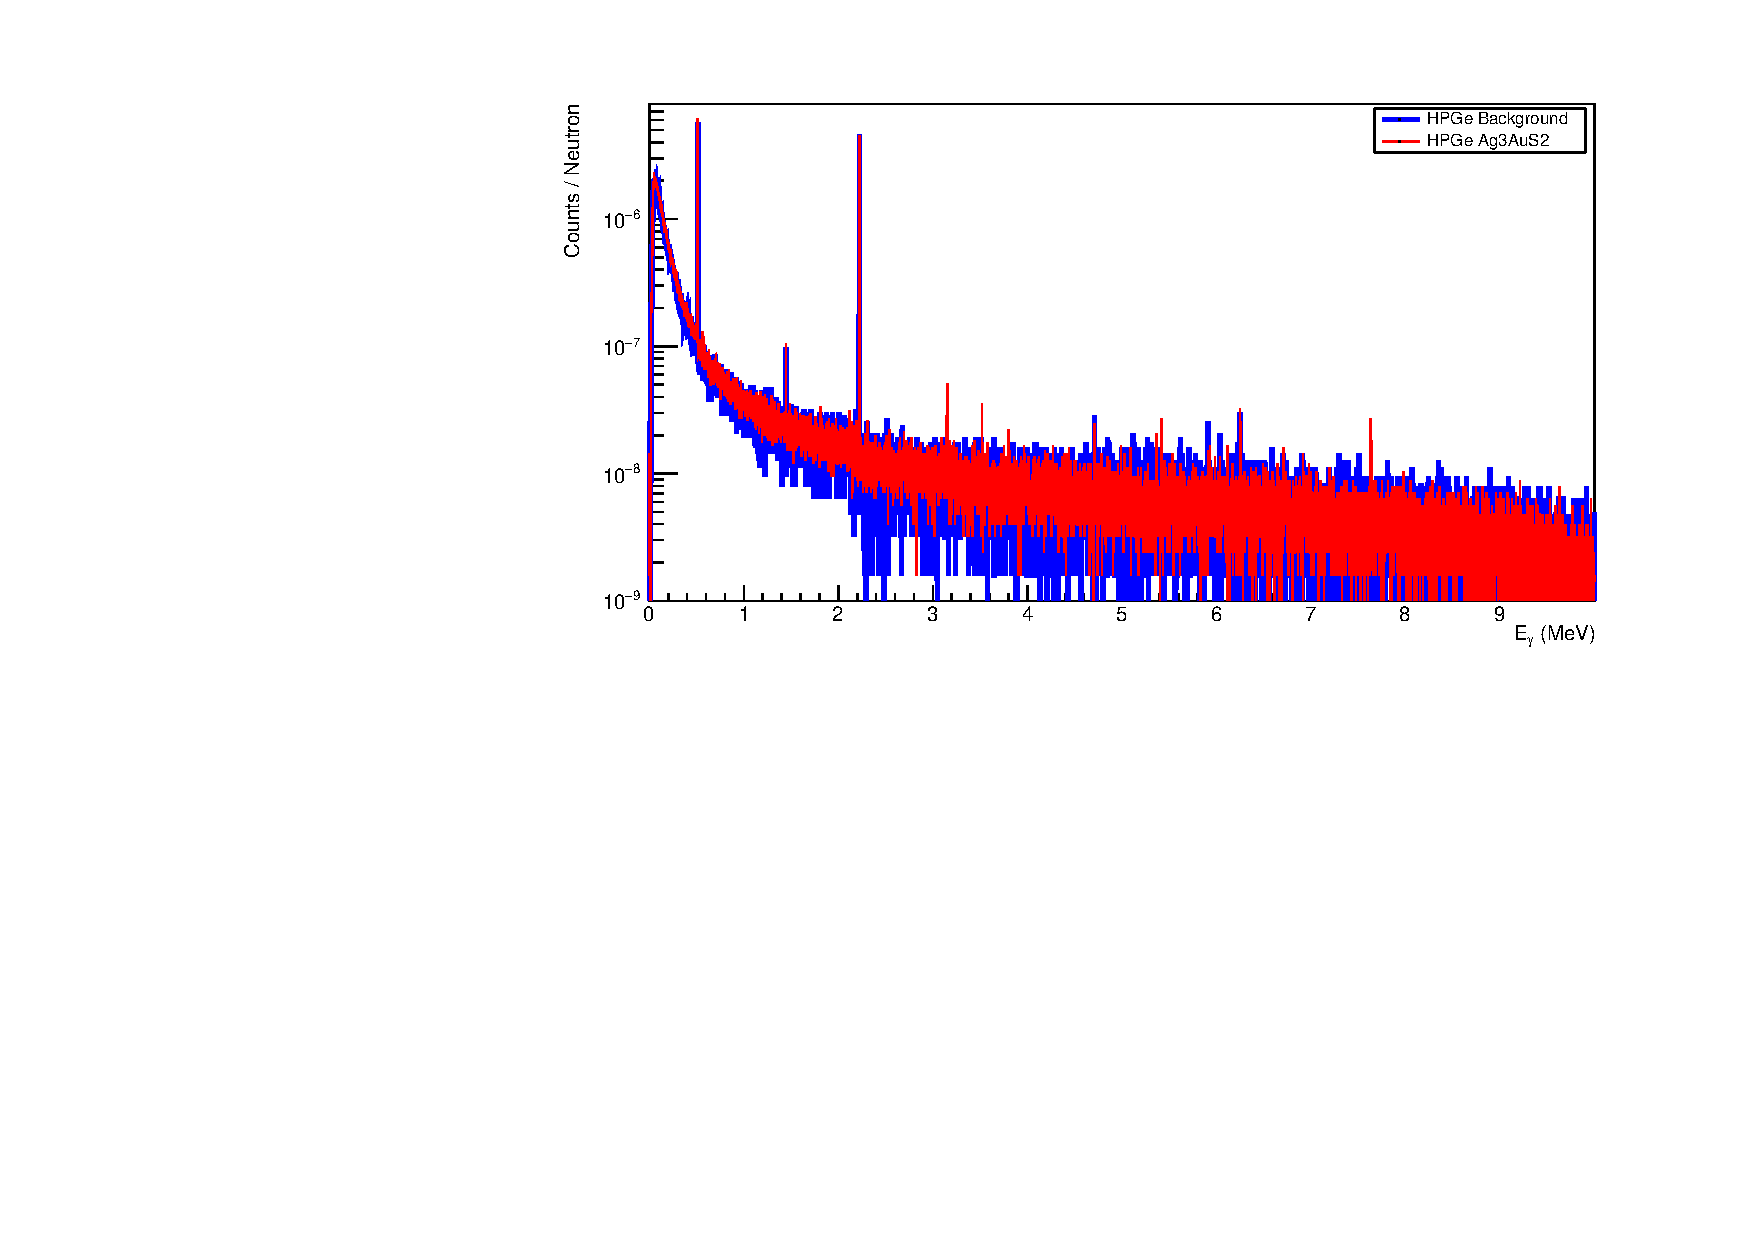
\includegraphics[width=1\textwidth]{res/smCuFeS2FonAll.pdf}
		\caption{Червоним - представлений спектр для $CuFeS_2$. Синім - фону} 
		\label{ris:CuFeS_2Fon}	
	\end{figure} 	
	В високо енергетичній частині спектру можна спостерігати пік для $S_2$
	
	\subsection{Аналіз спектру $U^{238}$}
	Було обрано збіднений уран, з наступним ізотопним складом $99.27\% -\  ^{238}U$, $ 0.72\% - \  ^{235}U$, $ 0.005\% - \ ^{234}U$, У ході набору було отримано наступний спектор Рис. ~\ref{ris:poorU}
	\begin{figure}[hbt!]
		%\vspace{-10pt}
		\centering 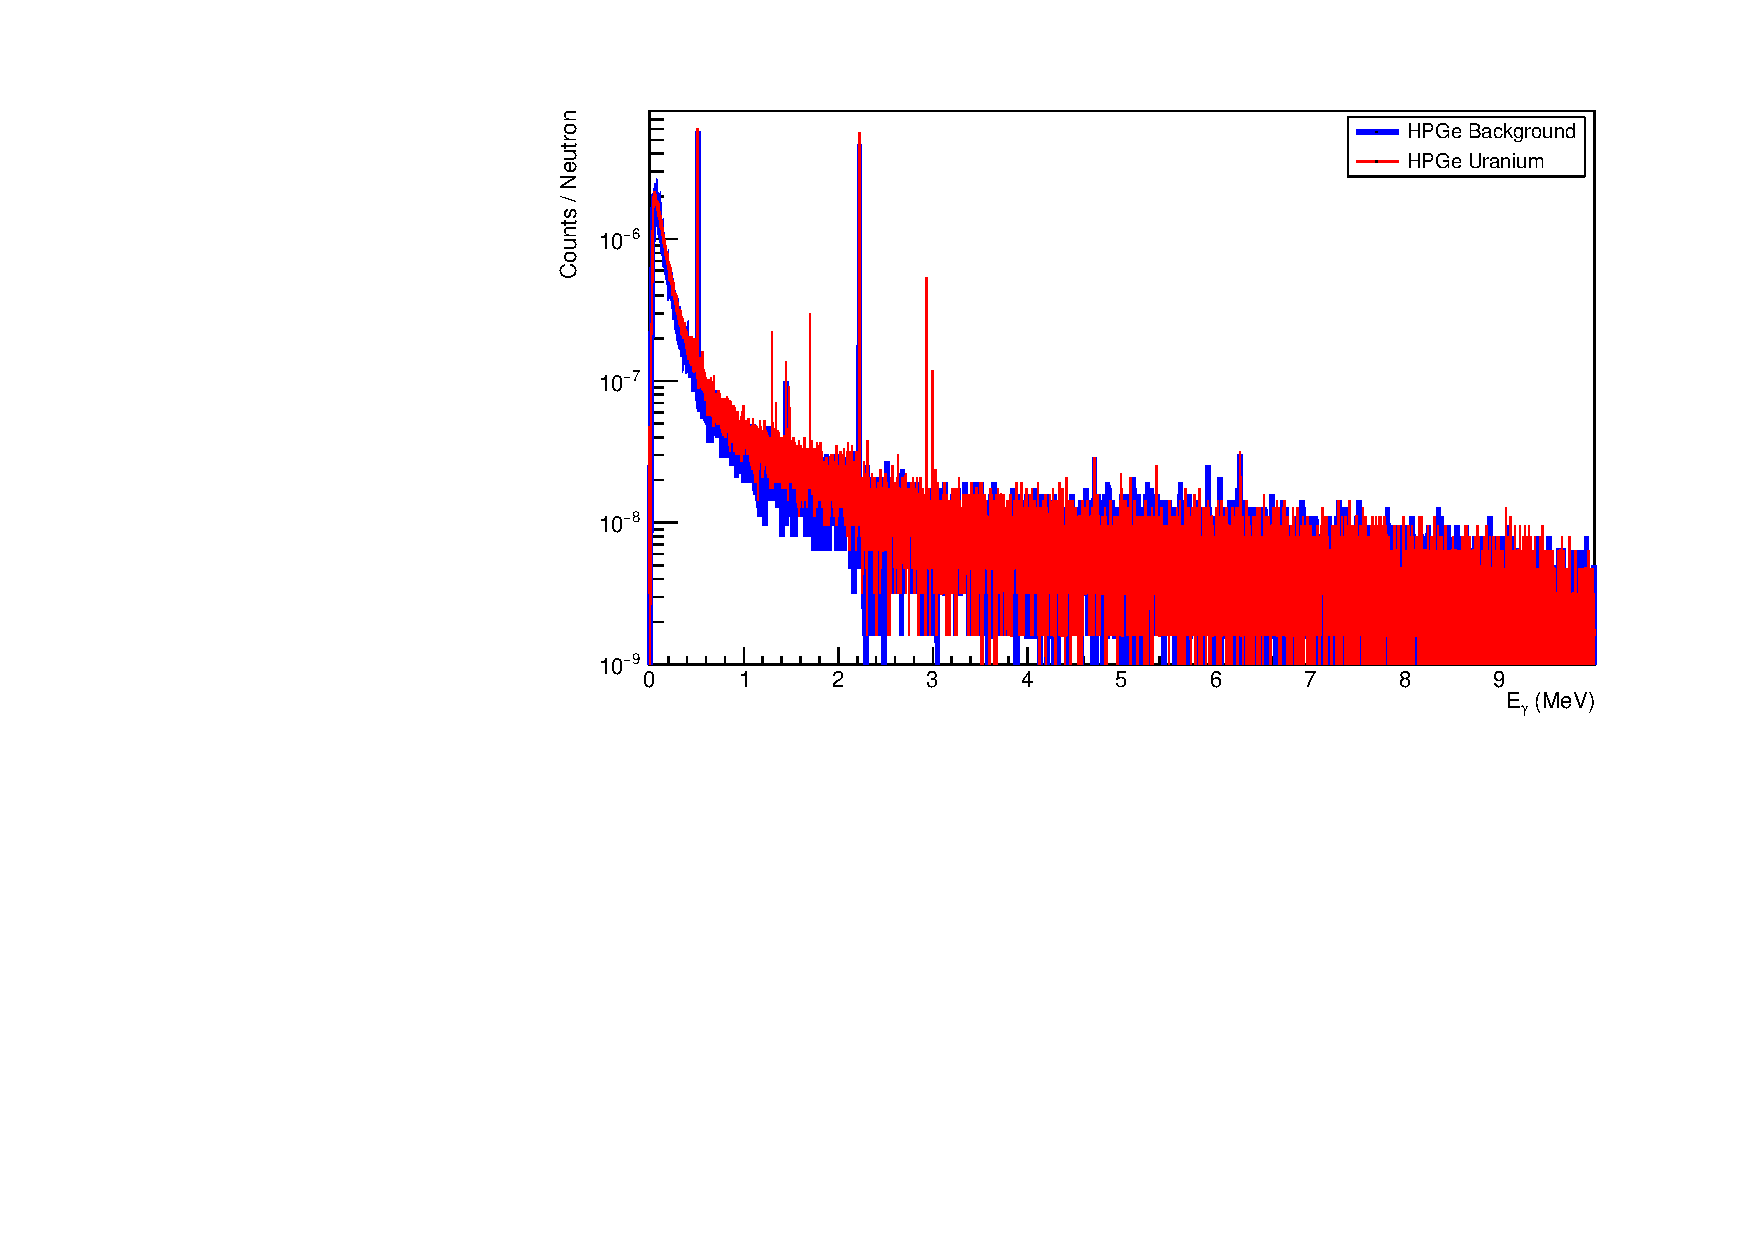
\includegraphics[width=1\textwidth]{res/poorUranium.pdf}
		\caption{Червоним - представлений спектр для $U^{238}$. Синім - фону} 
		\label{ris:poorU}	
	\end{figure} 	
	
	\newpage 
	\section{Висновки}
	\setcounter{figure}{0}
Метою даної роботи було створення моделі для детектування елементів що входять до складу корисних копалин на дні океану, та її валідація.
	
Для роботи було обрано ряд матеріалів, що входять до складу металічних руд.

Для кожного з даних матеріалів були набрані та проаналізовані спектри, та встановленні значення інтенсивності відносно фону. 

Модель успішно пройшла валідацію.  

Проведення набору спетрів для нейтронів різних енергій дало, можливість виявити та зареєструвати недоліки даної моделі та геометрії. 

На даному єтапі було проведено перевірку використання даної моделі для обмеженої кількості речовин. 

Встановлена відстань від джерела нейтронів до досліджуваної речовини може варіювати і бути більшою за 30 см. при енергіях нейтронів 14.2 МеВ.
	
	
\newpage 
\section{Додатки}
\setcounter{figure}{0}
\begin{figure}[h!]
	%\vspace{-10pt}
	\centering 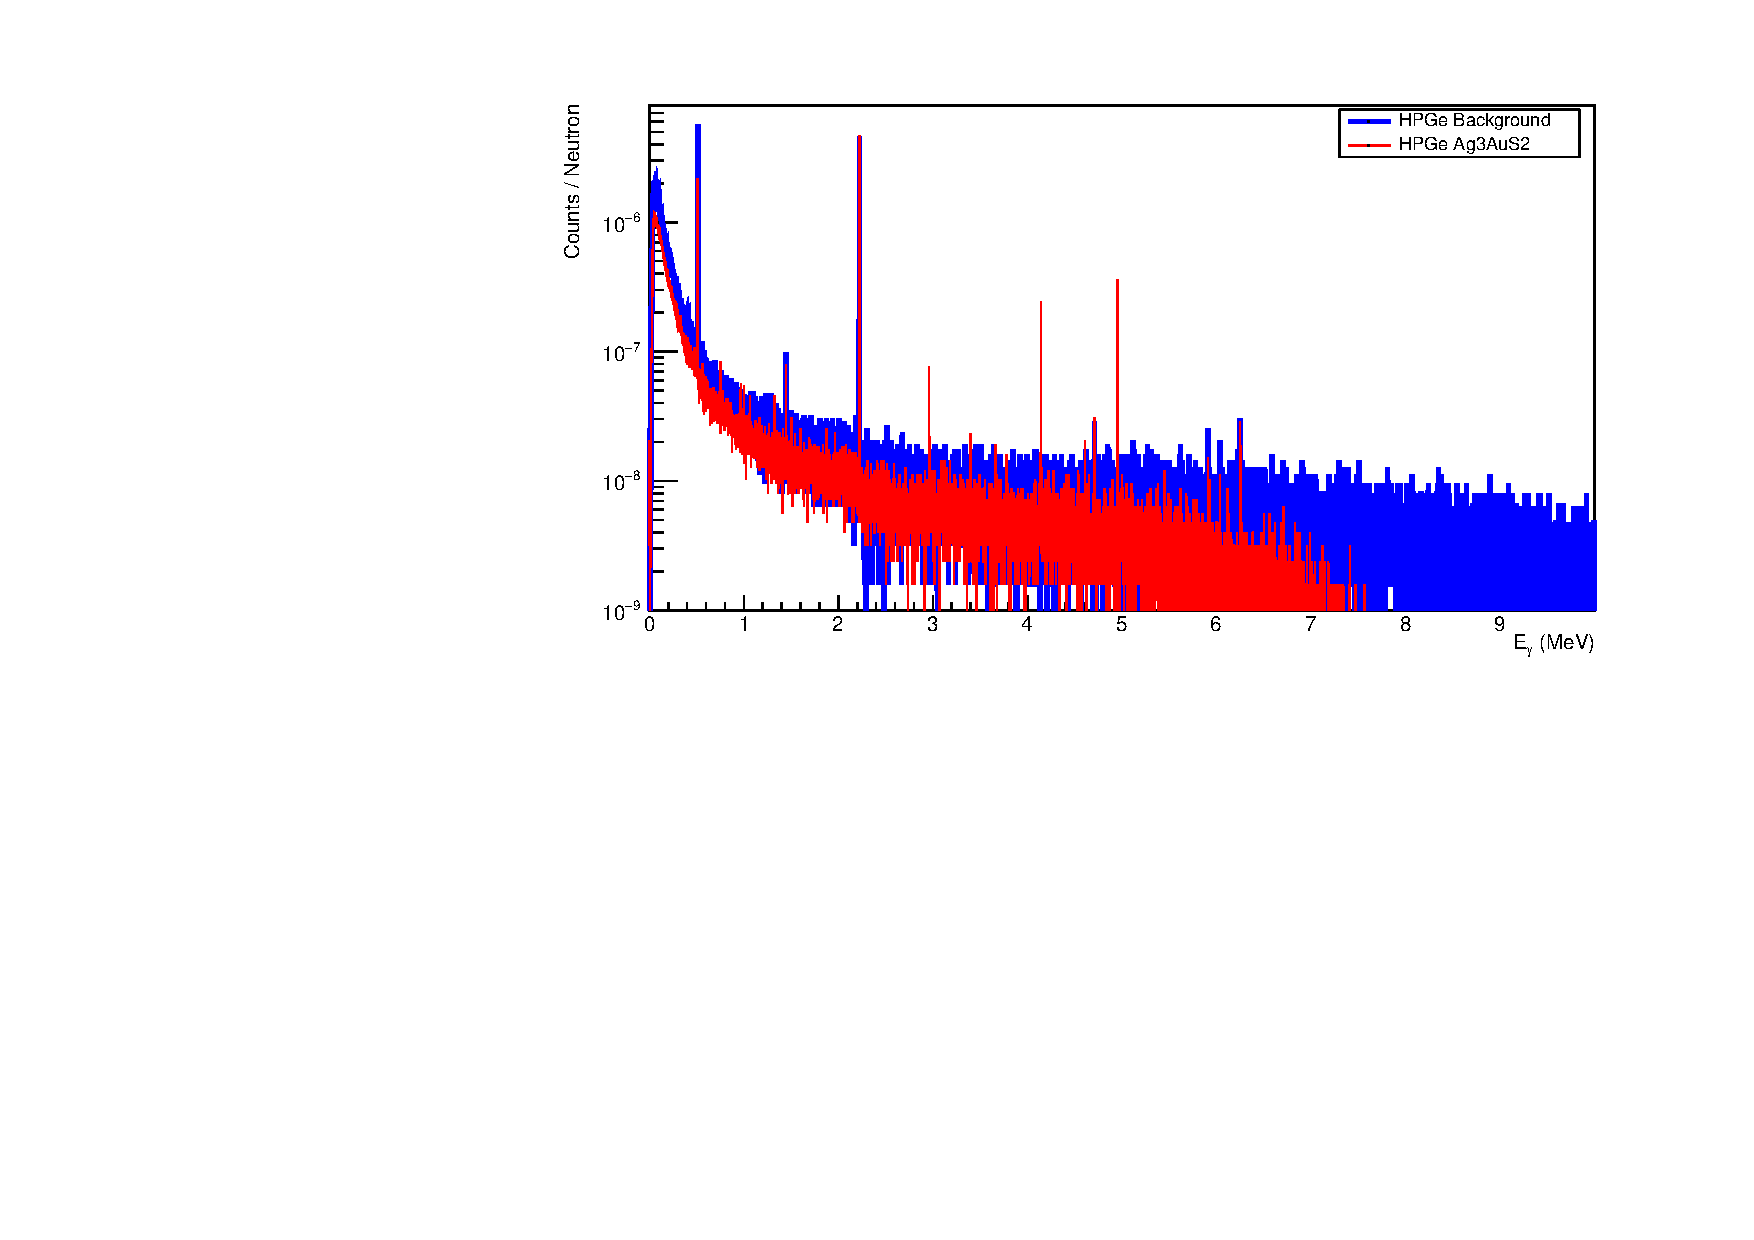
\includegraphics[width=1\textwidth]{res/Ag3AuS2_8_5MeVFonClasic.pdf}
	\caption{Червона - лінія спектру, набраного за опромінення нейтронами 8.5 МеВ}
	\label{ris:Ag3AuS28_5MeV}	
\end{figure} 
\begin{figure}[h!]
	%\vspace{-10pt}
	\centering 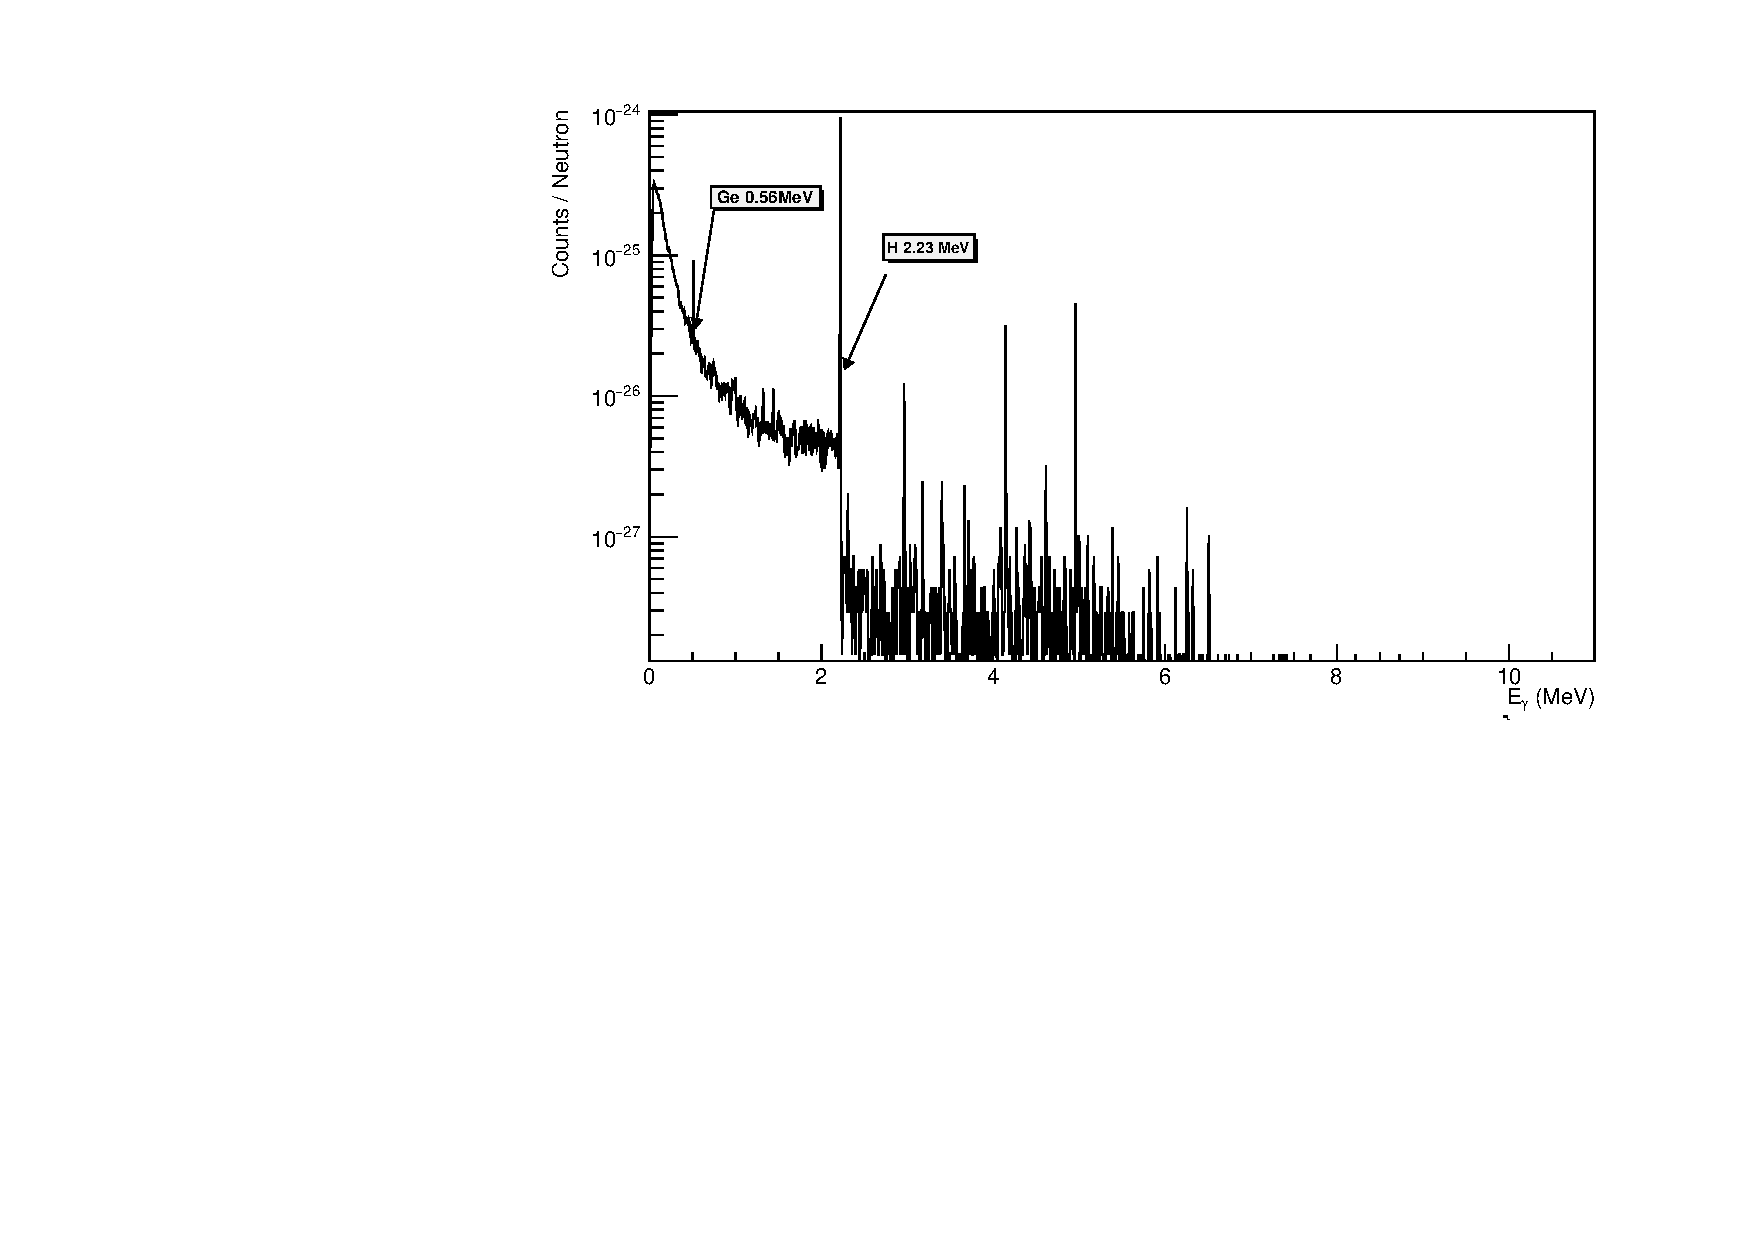
\includegraphics[width=1\textwidth]{res/AuAgS28MeV.pdf}
	\caption{Червона - лінія спектру, набраного за опромінення нейтронами 8.5 МеВ}
	\label{ris:Ag3AuS22_8MeV}	
\end{figure}
\begin{figure}[!]
	%\vspace{-10pt}
	\centering 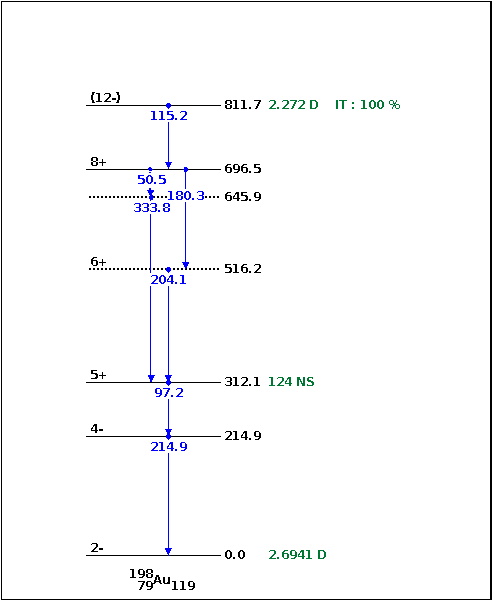
\includegraphics[width=1\textwidth]{images/au198levels.png}
	\caption{$Au^{198}$ Рівень $J\pi 12-$} 
	\label{ris:Au198Level12-}	
\end{figure} 
\begin{figure}[!]
	%\vspace{-10pt}
	\centering 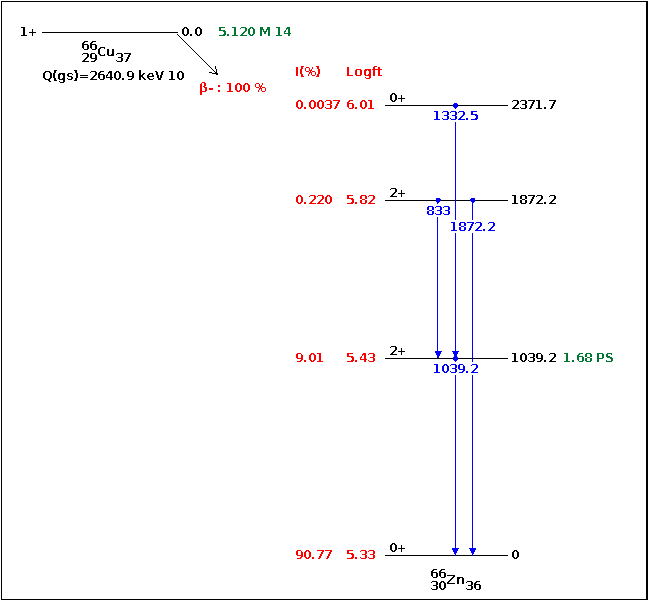
\includegraphics[width=1\textwidth]{images/cu66lbetadecay.png}
	\caption{$Cu^{66}_{29}(,\beta^-\  \tilde{\nu})Zn^{66}_{30}$ Схема розпаду та збудженні рівні $Zn^{66}$} 
	\label{ris:ZnLevels-}	
\end{figure} 

\pagebreak
\newpage	
%literature
\addcontentsline{toc}{section}{Література}
\begin{thebibliography}{}
	
	%	\comment{коментар: це джерело звідки були взяті розміри детектора}  
	\bibitem{1}\textit{M. Silarski, P. Sibczyński, Sz. Niedźwiecki, S. Sharma , J. Raj, P. Moskal Institute of Physics, Jagiellonian University, Lojasiewicza 11, 30-348 Kraków, Poland, National Centre for Nuclear Research, So ltana 7, 05-400 Otwock, Poland } Underwater detection of dangerous substances: status the
	SABAT project \label{lit:sabat}
	\bibitem{1} \textit{R.M. Keyser and T.R. Twomey} - Extended Source Sensitivity and Resolution Comparisons of Several HPGe Detector Types with Low-energy Capabilities 
	\bibitem{1} \textit{Aatos Heikkinen, Nikita Stepanov Helsinki Institute of Physics, P.O. Box 64, FIN-00014 University of Helsinki, Finland Johannes Peter Wellisch CERN, Geneva, Switzerland} - Bertini intra-nuclear cascade implementation in Geant4 
	\bibitem{1} \textit{Ю.В. Сереткин, Г.А. Пальянова Институт геологии и минералогии им. В.С. Соболева СО РАН} - ИЗОМОРФНОЕ ЗАМЕЩЕНИЕ СЕРЫ СЕЛЕНОМ И МОРФОТРОПНЫЙ ПЕРЕХОД В РЯДУ $Ag_3Au(Se,S)_2$ 	
	\bibitem{1} \textit{В. М. Округин1, А. У. Ким} О рудах Асачинского золото-серебряного месторождения
	(Южная Камчатка)
	\bibitem{1} \textit{Омельчук О.В., Загнітко В.М., Курило М.М.}ПОШУКИ ТА РОЗВІДКА РОДОВИЩ КОРИСНИХ КОПАЛИН КИЇВСЬКИЙ НАЦІОНАЛЬНИЙ УНІВЕРСИТЕТ ІМЕНІ ТАРАСА ШЕВЧЕНКА Навчально-науковий інститут «Інститут геології»
	\bibitem{1} \textit{Experimental Nuclear Reaction Data}
	\bibitem{1} \textit{O. A. Wasson, R. E. Chrien, M. R. Bhat, M. A. Lone, and M. Beer} $Au^{197}(n, \gamma)Au^{198}$ Reaction Mechanism 
	\bibitem{1} \textit{	I.A.Kondurov, A.I.Egorov, M.Kaminker, E.M.Korotkikh, A.M.Nikitin}  Neutron capture cross sections measurements for Co58m, Cu64, and Sc46
	\bibitem{1} \textit{ Geant4 Collaboration } Book For Application Developers
	Release 10.3
	\bibitem{1} \textit{ Alexander Howard, Gunter Folger, Jose Manuel Quesada, Vladimir Ivanchenko} Validation of Neutrons in Geant4 Using TARC Data - production, interaction and transportation \label{lit:tarc}
	\bibitem{1} \textit{H´ector Ren´e, Vega-Carrillo Celia, Torres-Muhech, Universidad Aut´onoma de Zacatecas}Low energy neutrons from a 239PuBe isotopic neutron source inserted inmoderating media
	\bibitem{1} \textit{Посилання на українську ассоціацію \href{http://www.clubofrome.org.ua/}{Римського Клубу}} \label{lit:romeClub}
	
\end{thebibliography}
	
\end{document}